\documentclass[a4paper]{article}

\usepackage{polski}
\usepackage[utf8]{inputenc}
\usepackage[pdftex]{graphicx}
\usepackage{fancyhdr}
\usepackage{float}

\newcommand{\prog}{\texttt}

\linespread{1.15}
\pagestyle{fancy}
\fancyhf{}
\chead{Specyfikacja implementacyjna}
\cfoot{Strona \thepage \ z \pageref{end}}

\title{Specyfikacja implementacyjna \\ Projekt \textit{Aplikacja OnePass} w języku Python}
\author{Jakub Czajka (299239)}

\begin{document}
\maketitle
\thispagestyle{empty}
\tableofcontents

\newpage

\section{Informacje ogólne}
\subsection{Ogólne parametry uruchomieniowe programu}
Język programowania: \textit{Python}.\medskip\\
Środowisko uruchomieniowe: \textit{dowolny system operacyjny obsługujący Pythona}.\medskip\\
Wielkość okna: \textit{1280 x 720 px}.\medskip\\
Położenie okna po uruchomieniu: \textit{środek ekranu}.

\subsection{Konwencja pisania kodu}
Kod programu będzie pisany zgodnie z poniższymi zasadami:
\begin{itemize}
    \item Kod pisany jest z poszanowaniem zasad czystego kodu.
    \item Nazwy są nazwami znaczącymi.
    \item Nazwy są pisane w języku angielskim.
    \item Nazwy klas są pisane w konwencji \textit{UpperCamelCase}.
    \item Nazwy metod i zmiennych są pisane małymi literami. Jeżeli składają się z kilku słów, słowa oddzielane są znakami \textit{"\_"}.
\end{itemize}

\section{Opis modułów i danych}
\subsection{Moduły w programie}
Nasz program jest podzielony na trzy odrębne moduły:

\subsubsection{Graficzny interfejs użytkownika}
Moduł ten odpowiedzialny jest za interaktywną i graficzną komunikację z użytkownikiem programu. Jego głównym zadaniem jest przedstawianie zawartości aplikacji oraz umożliwienie użytkownikowi komunikację z programem. Moduł ten połączony jest z modułem kontrolerów.

\subsubsection{Kontrolery}
Moduł ten odpowiedzialny jest za komunikację aplikacji między modułami. Łączy moduł graficznego interfejsu użytkownika z modułem obilczeń aplikacji.

\subsubsection{Obliczenia}
Moduł ten odpowiedzialny jest za pracę aplikacji. W tym miejscu przetwarzane są dane, wykonuje się szyfrowanie i deszyfrowanie oraz przechowuje się dane. Moduł ten komunikuje się z modułem kontrolerów.

\section{Opis klas}
\subsection{Model}

\subsubsection{MProfile}
\begin{description}
    \item[Pakiet:] model
    \item[Dziedziczy:] --
    \item[Konstruktor:] otrzymuje zmienne typu \prog{string} zawierające dane osobowe. Ustawia je w odpowiednie pola klasy.
    \item[Pola:] \hfill
    \begin{itemize}
        \item \prog{string name} -- przechowuje imię użytkownika.
        \item \prog{string surname} -- przechowuje nazwisko użytkownika.
        \item \prog{string email} -- przechowuje email użytkownika.
        \item \prog{string login} -- przechowuje login użytkownika.
        \item \prog{string hasło} -- przechowuje hasło użytkownika.
        \item \prog{List passwords} -- przechowuje obiekty haseł użytkownika.
        \item \prog{List notes} -- przechowuje notatki użytkownika.
    \end{itemize}
    \item[Metody:] \hfill
    \begin{itemize}
        \item \textbf{Prototyp:} \prog{public void update(string update)}\\\textbf{Zadanie:} z aktualizowanie informacji o uzytkowniku.
        \item \textbf{Prototyp:} \prog{public void update\_passwords(List update)}\\\textbf{Zadanie:} zaktualizowanie informacji o hasłach.
        \item \textbf{Prototyp:} \prog{public void update\_notes(List update)}\\\textbf{Zadanie:} Z aktualizowanie informacji o notatkach.
    \end{itemize}
\end{description}

\subsubsection{MPassword}
\begin{description}
    \item[Pakiet:] model
    \item[Dziedziczy:] --
    \item[Konstruktor:] otrzymuje zmienne typu \prog{string} zawierające dane hasła. Ustawia je w odpowiednie pola klasy.
    \item[Pola:] \hfill
    \begin{itemize}
        \item \prog{string name} -- przechowuje nazwę hasła.
        \item \prog{string login} -- przechowuje login.
        \item \prog{string password} -- przechowuje hasło.
        \item \prog{string url} -- przechowuje adres do strony.
        \item \prog{boolean is\_favourite} -- przechowuje wartość logiczną opisującą to czy element jest elementem \textit{ulubionym}.
    \end{itemize}
    \item[Metody:] \hfill
    \begin{itemize}
      \item \textbf{Prototyp:} \prog{public void update(string update)}\\\textbf{Zadanie:} zaktualizowanie informacji o obiekcie.
    \end{itemize}
\end{description}

\subsubsection{MNote}
\begin{description}
    \item[Pakiet:] model
    \item[Dziedziczy:] --
    \item[Konstruktor:] otrzymuje zmienne typu \prog{string} zawierające dane notatki. Ustawia je w odpowiednie pola klasy.
    \item[Pola:] \hfill
    \begin{itemize}
        \item \prog{string name} -- przechowuje nazwę pliku (nazwa notatki plus rozszerzenie).
        \item \prog{string text} -- przechowuje treść notatki.
    \end{itemize}
    \item[Metody:] \hfill
    \begin{itemize}
        \item \textbf{Prototyp:} \prog{public void update(string update)}\\\textbf{Zadanie:} zaktualizowanie danych notatki.
    \end{itemize}
\end{description}

\subsubsection{MHasher}
\begin{description}
    \item[Pakiet:] model
    \item[Dziedziczy:] --
    \item[Konstruktor:] bezargumentowy.
    \item[Pola:] brak
    \item[Metody:] \hfill
    \begin{itemize}
        \item \textbf{Prototyp:} \prog{public string hash(string msg)}\\\textbf{Zadanie:} haszuje podaną jako argument wiadomość.
    \end{itemize}
\end{description}

\subsubsection{MGenerator}
\begin{description}
    \item[Pakiet:] model
    \item[Dziedziczy:] --
    \item[Konstruktor:] bezargumentowy.
    \item[Pola:] brak
    \item[Metody:] \hfill
    \begin{itemize}
        \item \textbf{Prototyp:} \prog{public string generate(tuple parameters)}\\\textbf{Zadanie:} generuje hasło na podstawie kryteriów przekazanych jako argument w postaci krotki.
    \end{itemize}
\end{description}

\subsubsection{MChecker}
\begin{description}
    \item[Pakiet:] model
    \item[Dziedziczy:] --
    \item[Konstruktor:] bezargumentowy. Inicjuje pola.
    \item[Pola:] \hfill
    \begin{itemize}
        \item \prog{MHasher hasher} -- przechowuje obiekt typu \prog{MHasher}.
    \end{itemize}
    \item[Metody:] \hfill
    \begin{itemize}
        \item \textbf{Prototyp:} \prog{public boolean verify\_data(string data)}\\\textbf{Zadanie:} sprawdza poprawność podanego hasła. W tym celu wykorzystuje obiekt typu \prog{MHasher}.
    \end{itemize}
\end{description}

\subsubsection{MProfileMaker}
\begin{description}
    \item[Pakiet:] model
    \item[Dziedziczy:] --
    \item[Konstruktor:] bezargumentowy.
    \item[Pola:] \hfill
    \begin{itemize}
        \item \prog{MHasher hasher} -- przechowuje obiekt służący do zahaszowania hasła podanego przez użytkownika.
    \end{itemize}
    \item[Metody:] \hfill
    \begin{itemize}
        \item \textbf{Prototyp:} \prog{public boolean check\_data(string data)}\\\textbf{Zadanie:} sprawdza poprawność podanych danych przy rejestracji.
        \item \textbf{Prototyp:} \prog{private string hash\_password(string password)}\\\textbf{Zadanie:} hashuje podane jako argument hasło.
        \item \textbf{Prototyp:} \prog{private MProfile make\_profile()}\\\textbf{Zadanie:} utworzenie nowego obiektu typu \prog{MProfile} z danych podanych przy rejestracji.
    \end{itemize}
\end{description}

\subsubsection{MLoader}
\begin{description}
    \item[Pakiet:] model
    \item[Dziedziczy:] --
    \item[Konstruktor:] bezargumentowy.
    \item[Pola:] \hfill
    \begin{itemize}
        \item \prog{List files} -- przechowuje listę nazw plików zaszyfrowanych.
        \item \prog{List notes} -- przechowuje listę nazw notatek zaszyfrowanych.
    \end{itemize}
    \item[Metody:] \hfill
    \begin{itemize}
        \item \textbf{Prototyp:} \prog{public void load\_logins()}\\\textbf{Zadanie:} załadowuje plik z loginami do programu.
        \item \textbf{Prototyp:} \prog{public MProfile load\_profiles()}\\\textbf{Zadanie:} załadowuje plik z profilem do programu.
    \end{itemize}
\end{description}

\subsubsection{MEncryptor}
\begin{description}
    \item[Pakiet:] model
    \item[Dziedziczy:] --
    \item[Konstruktor:] bezargumentowy.
    \item[Pola:] \hfill
    \begin{itemize}
        \item \prog{List notes} -- przechowuje listę nazw plików z notatkami
        \item \prog{List passwords} -- przechowuje listę haseł do zaszyfrowania.
        \item \prog{MProfile profile} -- przechowuje obiekt zawierający informacje o profilu.
    \end{itemize}
    \item[Metody:] \hfill
    \begin{itemize}
        \item \textbf{Prototyp:} \prog{public string decrypt(string file)}\\\textbf{Zadanie:} rozszyfrowuje podany plik.
        \item \textbf{Prototyp:} \prog{public string encrypt(string file)}\\\textbf{Zadanie:} szyfruje podany łańcuch.
    \end{itemize}
\end{description}

\subsection{Presenter}
Pakiet \textit{Presenter} zawiera klasy odpowiadające za sterowanie ekranami i połączenie z pakietem \textit{Model}. Działanie większość metod klas znajdujących się w tym pakiecie sprowadza się do reakcji na naciśnięty przycisk w GUI.\\
Każda klasa ma w sobie pola ekranów które może wyświetlić.
\subsubsection{PMainWin}
\textit{<<klasa abstrakcyjna>>}
\begin{description}
    \item[Pakiet:] presenter
    \item[Dziedziczy:] --
    \item[Konstruktor:] bezargumentowy.
    \item[Pola:]brak
    \item[Metody:] \hfill
    \begin{itemize}
        \item \textbf{Prototyp:} \prog{public void encrypt\_file\_button\_handle()}\\\textbf{Zadanie:} zmienia bieżącą scenę na ekran szyfrowania plików podanych przez użytkownika.
        \item \textbf{Prototyp:} \prog{public void generate\_button\_handle()}\\\textbf{Zadanie:} zmienia bieżącą scenę na ekran generowania hasła.
        \item \textbf{Prototyp:} \prog{public void home\_button\_handle()}\\\textbf{Zadanie:} zmienia bieżącą scenę na ekran główny po zalogowaniu.
        \item \textbf{Prototyp:} \prog{public void note\_button\_handle()}\\\textbf{Zadanie:} zmienia bieżącą scenę na ekran z listą notatek.
        \item \textbf{Prototyp:} \prog{public void password\_button\_handle()}\\\textbf{Zadanie:} zmienia bieżącą scenę na ekran z listą haseł.
    \end{itemize}
\end{description}
Klasa \prog{PMainWin} jest klasą abstrakcyjną, po której dziedziczą następujące klasy:
\begin{itemize}
    \item PMainWinAfter
    \item PPasswordListWin
    \item PNoteListWin
    \item PEncryptWin
\end{itemize}

\subsubsection{PMainWinBefore}
\begin{description}
    \item[Pakiet:] presenter
    \item[Dziedziczy:] --
    \item[Konstruktor:] bezargumentowy. Inicjuje pola.
    \item[Pola:] \hfill
    \begin{itemize}
        \item \prog{MLoader loader} -- przechowuje obiekty załadowujący loginy.
        \item \prog{string logins} -- pole przechowujące załadowane loginy.
    \end{itemize}
    \item[Metody:] \hfill
    \begin{itemize}
        \item Metody odpowiedzialne za reakcje na kliknięcie przycisku:
        \begin{itemize}
            \item about\_app\_button\_handle()
            \item sign\_up\_button\_handle()
            \item sign\_in\_button\_handle()
            \item generate\_button\_handle()
        \end{itemize}
        \item \textbf{Prototyp:} \prog{private string load\_logins()}\\\textbf{Zadanie:} wpisanie w pole \prog{logins} pliku z loginami.
    \end{itemize}
\end{description}

\subsubsection{PSignInWin}
\begin{description}
    \item[Pakiet:] presenter
    \item[Dziedziczy:] --
    \item[Konstruktor:] bezargumentowy. Inicjuje pola.
    \item[Pola:] \hfill
    \begin{itemize}
        \item \prog{MProfile profile} -- przechowuje obiekt profilu.
        \item \prog{string logins} -- pole przechowujące załadowane loginy.
        \item \prog{MLoader loader} -- pole przechowujące załadowujący profil.
        \item \prog{MChecker checker} -- pole przechowujące obiekt sprawdzający poprawność danych.
    \end{itemize}
    \item[Metody:] \hfill
    \begin{itemize}
        \item Metody odpowiedzialne za reakcje na kliknięcie przycisku:
        \begin{itemize}
            \item forget\_button\_handle()
            \item sign\_up\_button\_handle()
            \item sign\_in\_button\_handle()
        \end{itemize}
        \item \textbf{Prototyp:} \prog{private void validate\_data(string data)}\\\textbf{Zadanie:} wywołuje metodę sprawdzającą poprawność danych.
        \item \textbf{Prototyp:} \prog{private void validate\_data(string data)}\\\textbf{Zadanie:} wywołuje metodę sprawdzającą poprawność danych.
        \item \textbf{Prototyp:} \prog{private void load\_profile(string data)}\\\textbf{Zadanie:} wywołuje metodę pobierającą dane, deszyfrującą je i tworzy obiekt typu \prog{MProfile}.
    \end{itemize}
\end{description}

\subsubsection{PSignUpWin}
\begin{description}
    \item[Pakiet:] presenter
    \item[Dziedziczy:] --
    \item[Konstruktor:] bezargumentowy. Inicjuje pola.
    \item[Pola:] \hfill
    \begin{itemize}
        \item \prog{MProfileMaker profile\_maker} -- przechowuje obiekt tworzący profil.
    \end{itemize}
    \item[Metody:] \hfill
    \begin{itemize}
        \item Metody odpowiedzialne za reakcje na kliknięcie przycisku:
        \begin{itemize}
            \item sign\_up\_button\_handle()
        \end{itemize}
        \item \textbf{Prototyp:} \prog{private void validate\_data(string data)}\\\textbf{Zadanie:} wywołuje metodę sprawdzającą poprawność danych.
    \end{itemize}
\end{description}

\subsubsection{PGenerateWin}
\begin{description}
    \item[Pakiet:] presenter
    \item[Dziedziczy:] --
    \item[Konstruktor:] bezargumentowy. Inicjuje pola.
    \item[Pola:] \hfill
    \begin{itemize}
        \item \prog{MGenerator generator} -- przechowuje obiekt generujący hasła.
        \item \prog{VGenerateWin generate\_win} -- przechowuje obiekt okna generacji.
    \end{itemize}
    \item[Metody:] \hfill
    \begin{itemize}
        \item Metody odpowiedzialne za reakcje na kliknięcie przycisku:
        \begin{itemize}
            \item generate\_button\_handle(tuple parameters)
        \end{itemize}
    \end{itemize}
\end{description}

\subsubsection{PPasswordListWin}
\begin{description}
    \item[Pakiet:] presenter
    \item[Dziedziczy:] --
    \item[Konstruktor:] bezargumentowy. Inicjuje pola.
    \item[Pola:] \hfill
    \begin{itemize}
        \item \prog{MProfile profile} -- przechowuje obiekt zwierający informacje o profilu.
    \end{itemize}
    \item[Metody:] \hfill
    \begin{itemize}
        \item Metody odpowiedzialne za reakcje na kliknięcie przycisku:
        \begin{itemize}
            \item add\_button\_handle()
            \item choose\_button\_handle()
        \end{itemize}
    \end{itemize}
\end{description}

\subsubsection{PPasswordWin}
\begin{description}
    \item[Pakiet:] presenter
    \item[Dziedziczy:] --
    \item[Konstruktor:] bezargumentowy. Inicjuje pola.
    \item[Pola:] \hfill
    \begin{itemize}
        \item \prog{MPassword password} -- przechowuje obiekt zwierający hasło.
    \end{itemize}
    \item[Metody:] \hfill
    \begin{itemize}
        \item Metody odpowiedzialne za reakcje na kliknięcie przycisku:
        \begin{itemize}
            \item save\_button\_handle()
            \item show\_button\_handle()
        \end{itemize}
        \item \textbf{Prototyp:} \prog{private void update(List passwords)}\\\textbf{Zadanie:} aktualizuje listę haseł.
    \end{itemize}
\end{description}

\subsubsection{PAddPasswordWin}
\begin{description}
    \item[Pakiet:] presenter
    \item[Dziedziczy:] --
    \item[Konstruktor:] bezargumentowy. Inicjuje pola.
    \item[Pola:] \hfill
    \begin{itemize}
        \item \prog{MPassword password} -- przechowuje obiekt zwierający hasło.
        \item \prog{MProfile profile} -- przechowuje obiekt zawierający informacje o profilu.
    \end{itemize}
    \item[Metody:] \hfill
    \begin{itemize}
        \item Metody odpowiedzialne za reakcje na kliknięcie przycisku:
        \begin{itemize}
            \item save\_button\_handle()
            \item generate\_button\_handle()
        \end{itemize}
    \end{itemize}
\end{description}

\subsubsection{PNoteListWin}
\begin{description}
    \item[Pakiet:] presenter
    \item[Dziedziczy:] --
    \item[Konstruktor:] bezargumentowy. Inicjuje pola.
    \item[Pola:] \hfill
    \begin{itemize}
        \item \prog{MEncryptor encryptor} -- przechowuje obiekt zawierający metody do szyfrowania i deszyfrowania.
        \item \prog{MLoader loader} -- przechowuje obiekt zawierający pole z wczytanymi nazwami plików.
    \end{itemize}
    \item[Metody:] \hfill
    \begin{itemize}
        \item Metody odpowiedzialne za reakcje na kliknięcie przycisku:
        \begin{itemize}
            \item encrypt\_button\_handle()
            \item decrypt\_button\_handle()
        \end{itemize}
    \end{itemize}
\end{description}

\subsection{View}
Pakiet ten zawiera klasy odpowiedzialne za wygląd okien aplikacji. Każda z tych klas ma metody odpowiedzialne za reagowanie na akcję. Dodatkowo jedynymi polami jakie przechowują te klasy są elementy GUI oraz kontroler.

\section{Budowa GUI}
\subsection{Opis pól i słuchaczy}
\subsubsection{Ekran startowy}
\begin{itemize}
    \item \prog{ImageView newGameButton} -- przechwytywacz zdarzenia typu kliknięcie lewego przycisku myszy, zmiana sceny.
    \item \prog{ImageView loadGameButton} -- przechwytywacz zdarzenia typu kliknięcie lewego przycisku myszy, zmiana sceny.
    \item \prog{ImageView aboutGameButton} -- przechwytywacz zdarzenia typu kliknięcie lewego przycisku myszy, zmiana sceny.
\end{itemize}

\subsubsection{Ekran wprowadzania imion graczy}
\begin{itemize}
    \item \prog{TextField playerOneTextField} -- przechwytywacz zdarzenia typu wykonana akcja, ustawienie zmiennej w obiekcie Ship.
    \item \prog{TextField playerTwoTextField} -- przechwytywacz zdarzenia typu wykonana akcja, ustawienie zmiennej w obiekcie Ship.
    \item \prog{ImageView nextButton} -- przechwytywacz zdarzenia typu kliknięcie lewego przycisku myszy, zmiana sceny.
\end{itemize}

\subsubsection{Ekran wczytywania gry}
\begin{itemize}
    \item \prog{ImageView nextButton} -- przechwytywacz zdarzenia typu kliknięcie lewego przycisku myszy, wywołanie metody odpowiedzialnej za wczytanie stanu gry i zmiana sceny.
\end{itemize}

\subsubsection{Ekran o grze}
\begin{itemize}
    \item \prog{ImageView backButton} -- przechwytywacz zdarzenia typu kliknięcie lewego przycisku myszy, zmiana sceny.
\end{itemize}

\subsubsection{Ekran gry}
\begin{itemize}
    \item \prog{ImageView saveGameButton} -- przechwytywacz zdarzenia typu kliknięcie lewego przycisku myszy, wywołanie metody odpowiedzialnej za zapis stanu gry.
    \item \prog{ImageView pauseGameButton} -- przechwytywacz zdarzenia typu kliknięcie lewego przycisku myszy, zawieszenie działania programu i zmiana sceny.
\end{itemize}

\subsubsection{Ekran zatrzymania gry}
\begin{itemize}
    \item \prog{ImageView resumeGameButton} -- przechwytywacz zdarzenia typu kliknięcie lewego przycisku myszy, wznowienie pracy programu i zmiana sceny.
    \item \prog{ImageView saveGameButton} -- przechwytywacz zdarzenia typu kliknięcie lewego przycisku myszy, wywołanie metody odpowiedzialnej za zapis stanu gry.
    \item \prog{ImageView quitGameButton} -- przechwytywacz zdarzenia typu kliknięcie lewego przycisku myszy, zmiana sceny.
\end{itemize}

\subsubsection{Ekran wygranej}
\begin{itemize}
    \item \prog{ImageView playAgainButton} -- przechwytywacz zdarzenia typu kliknięcie lewego przycisku myszy, zmiana sceny i rozpoczęcie nowej rozgrywki.
    \item \prog{ImageView quitButton} -- przechwytywacz zdarzenia typu kliknięcie lewego przycisku myszy, zakończenie działania programu.
\end{itemize}

\subsubsection{Ekran przegranej}
\begin{itemize}
    \item \prog{ImageView playAgainButton} -- przechwytywacz zdarzenia typu kliknięcie lewego przycisku myszy, zmiana sceny i rozpoczęcie nowej rozgrywki.
    \item \prog{ImageView quitButton} -- przechwytywacz zdarzenia typu kliknięcie lewego przycisku myszy, zakończenie działania programu.
\end{itemize}

\subsection{Budowa wewnętrzna GUI}
Na poniższych rysunkach przedstawiających główne ekrany programu można zaobserwować podział poszczególnych scen na panele i stopień ich zagnieżdżenia.
\begin{figure}[H]
    \centering
    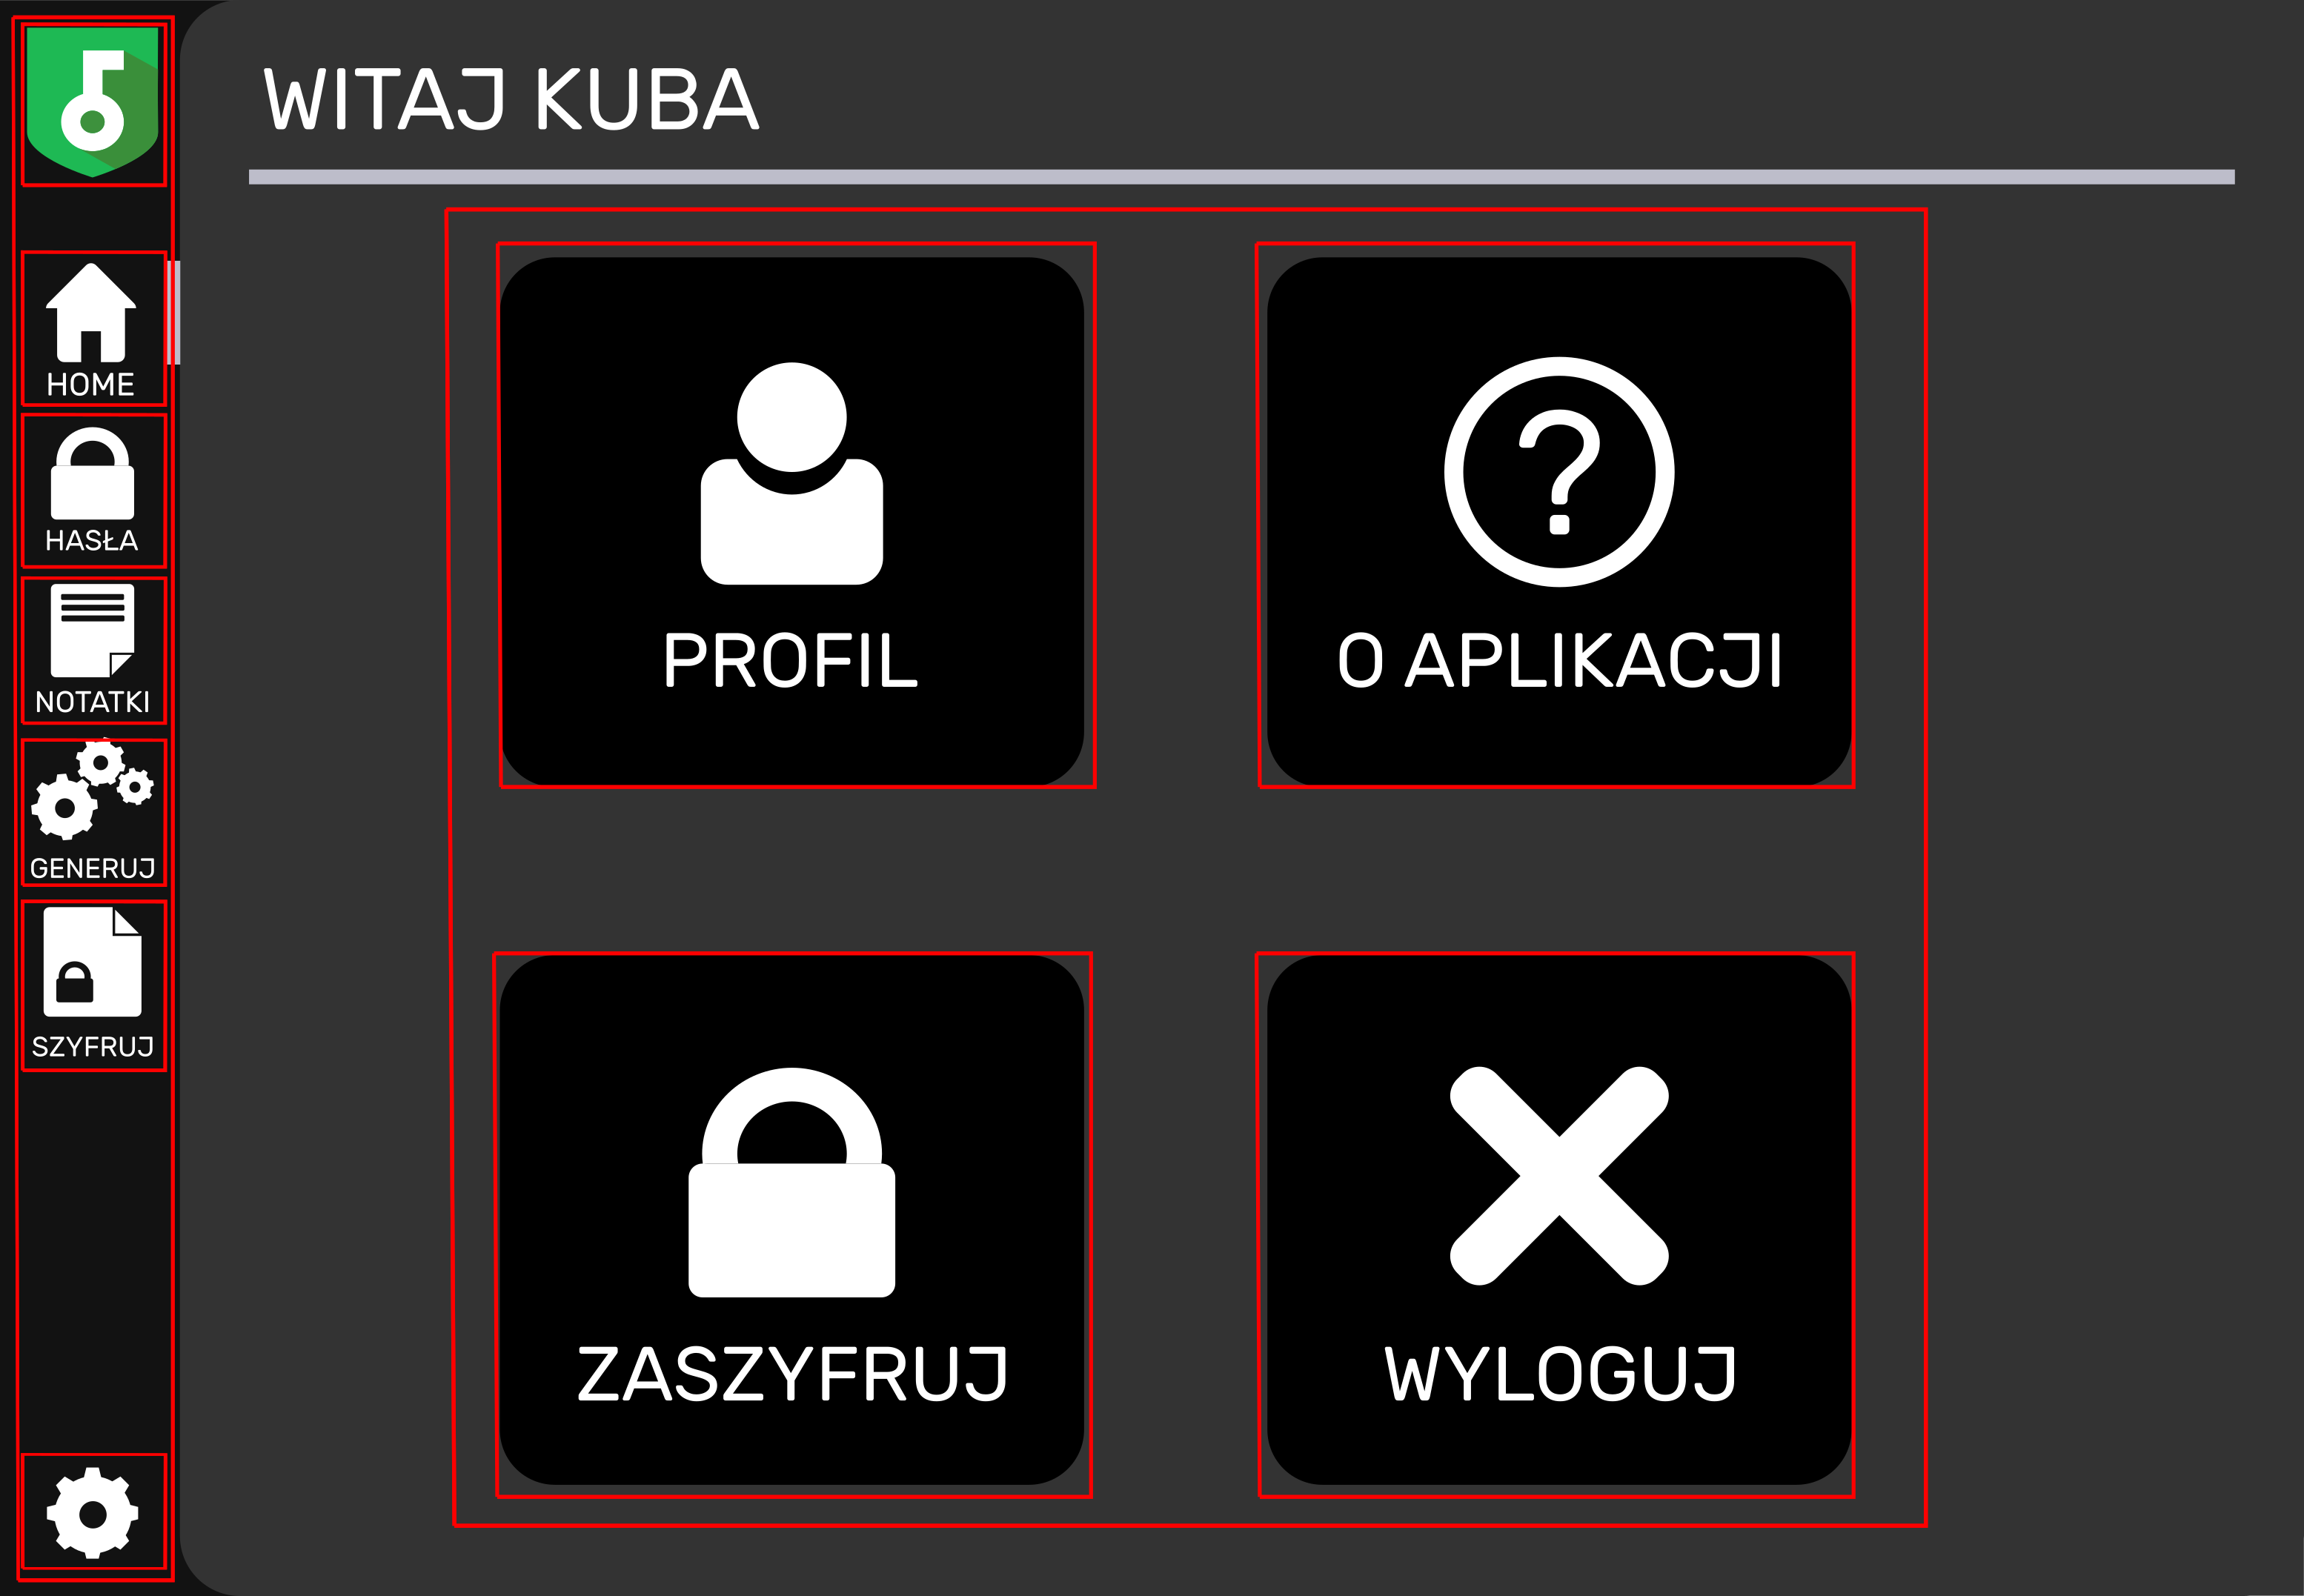
\includegraphics[width=1\textwidth]{img/ekran_przed_zalogowanie.png}
    \caption{Ekran startowy -- przed zalogowaniem}
    \label{fig:startPrzed}
\end{figure}

\begin{figure}[H]
    \centering
    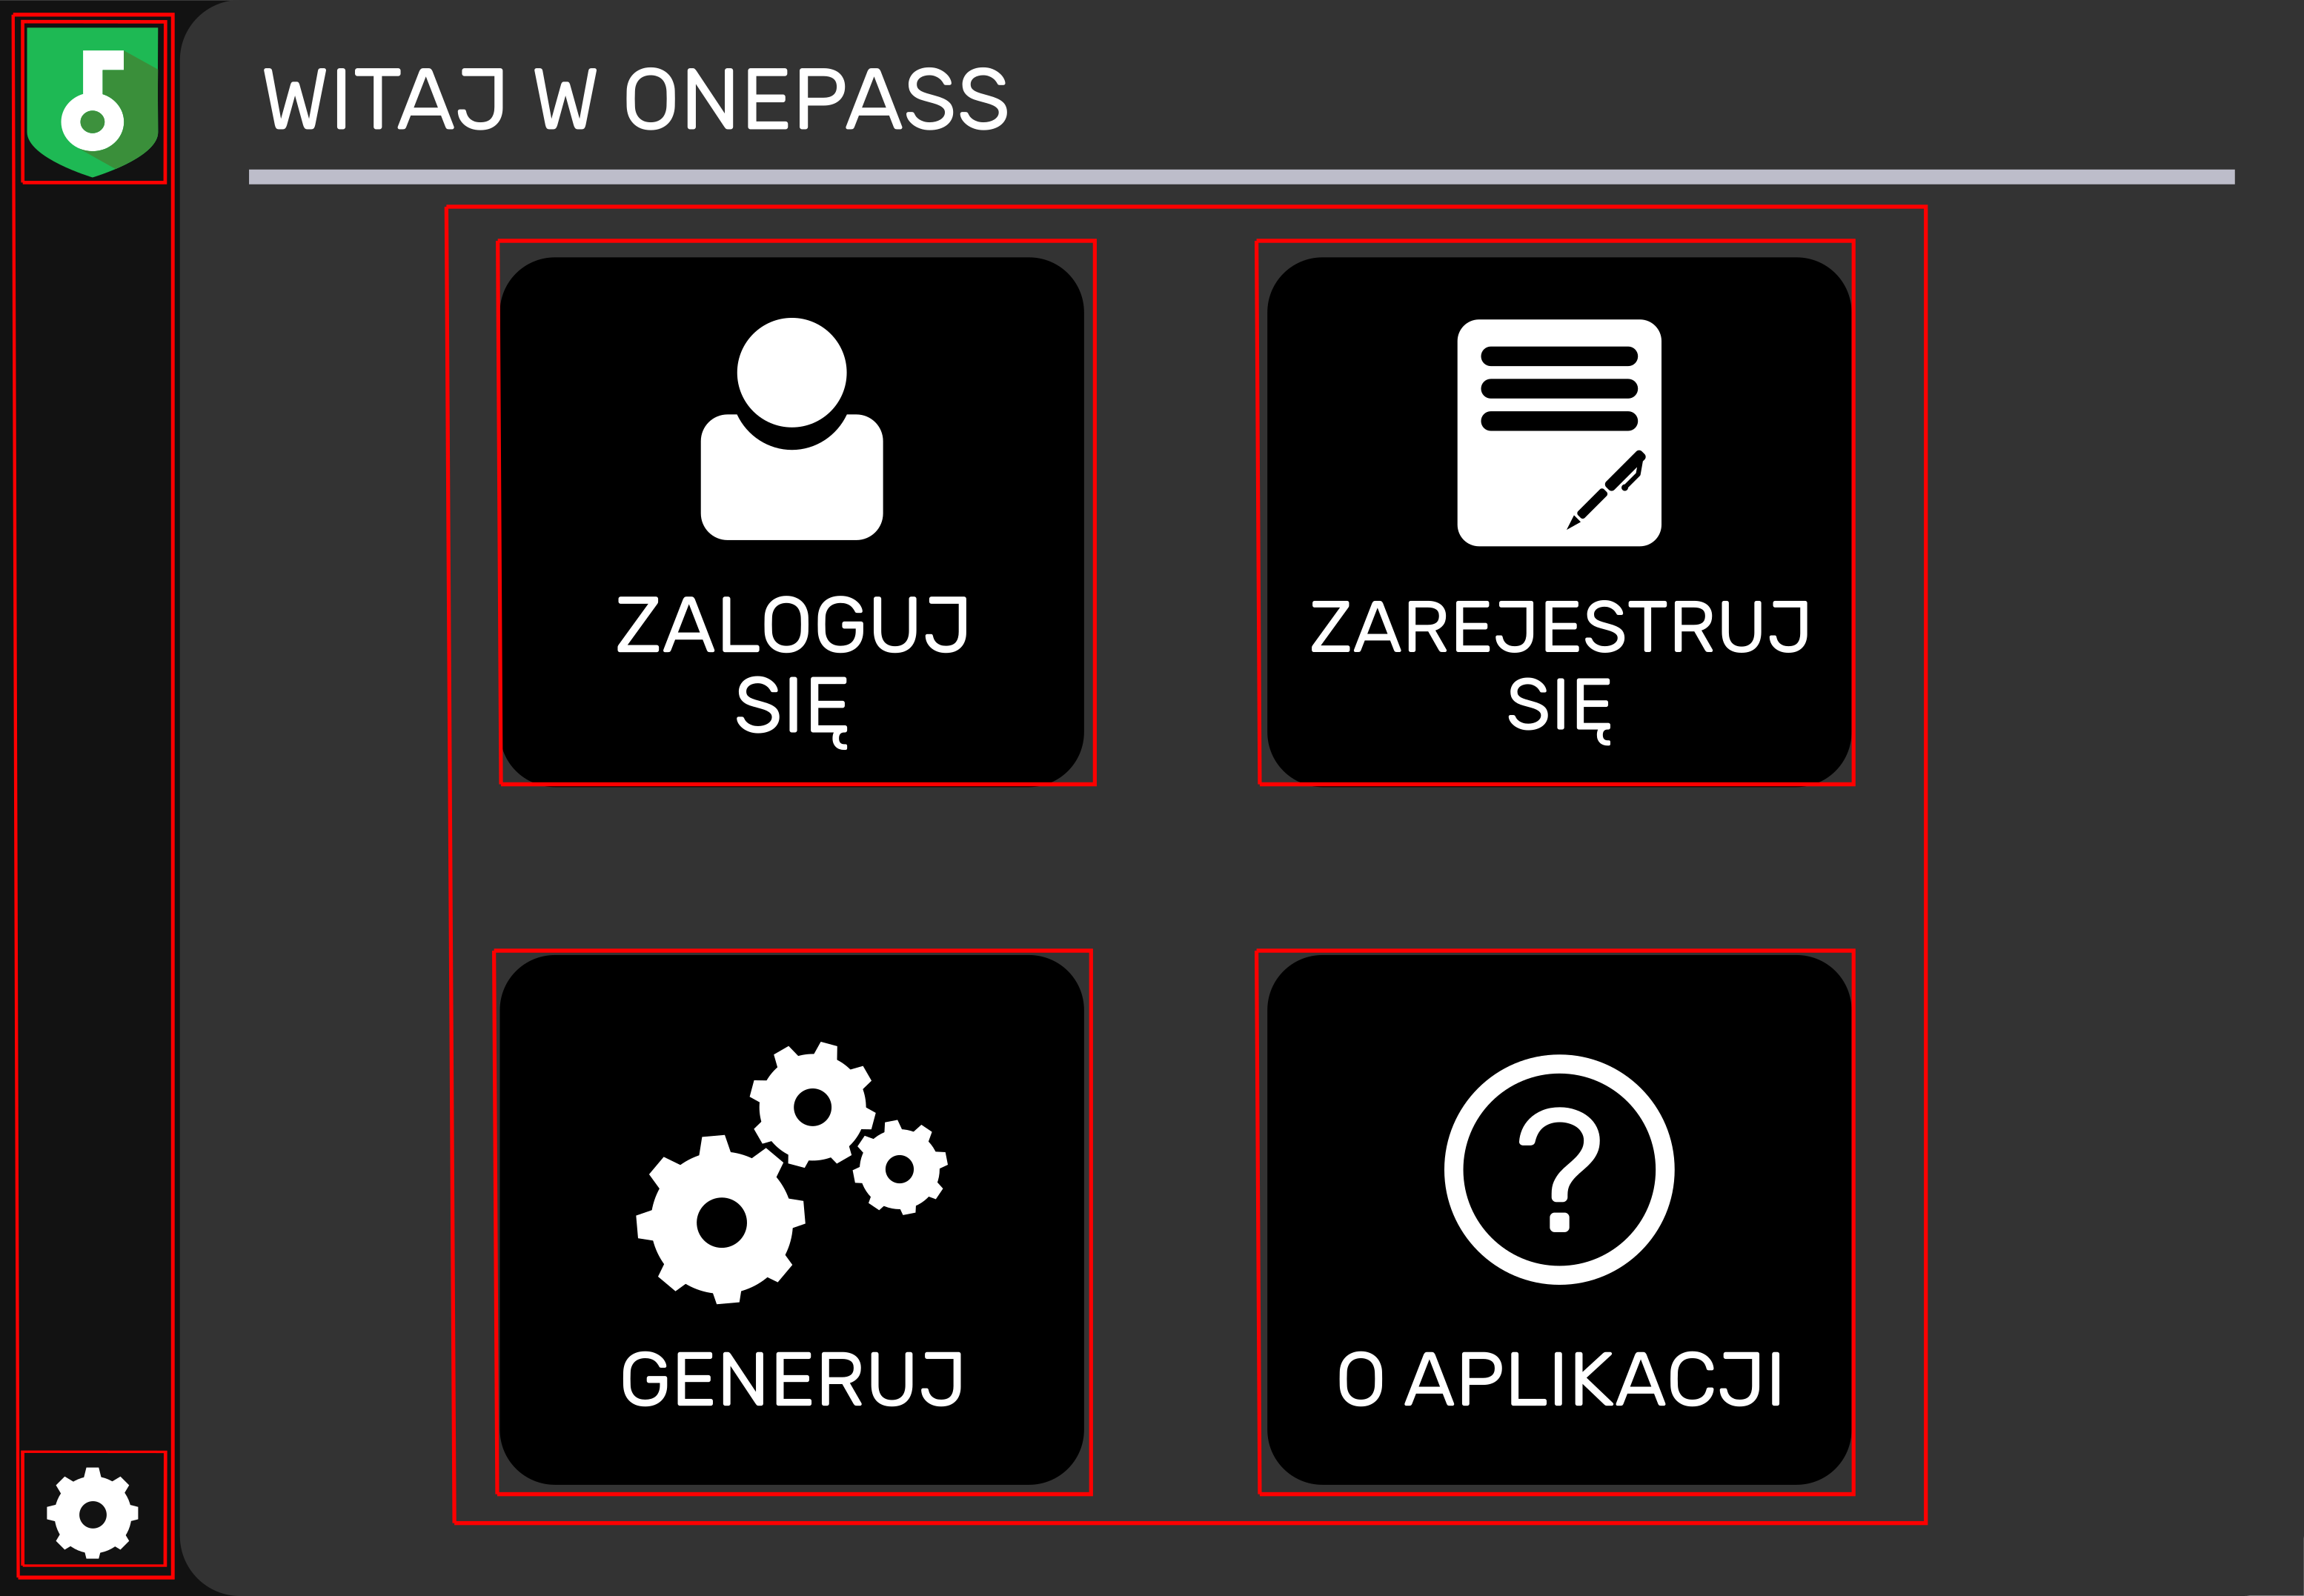
\includegraphics[width=1\textwidth]{img/ekran_po_zalogowanie.png}
    \caption{Ekran startowy -- po zalogowaniu}
    \label{fig:startPo}
\end{figure}

\begin{figure}[H]
    \centering
    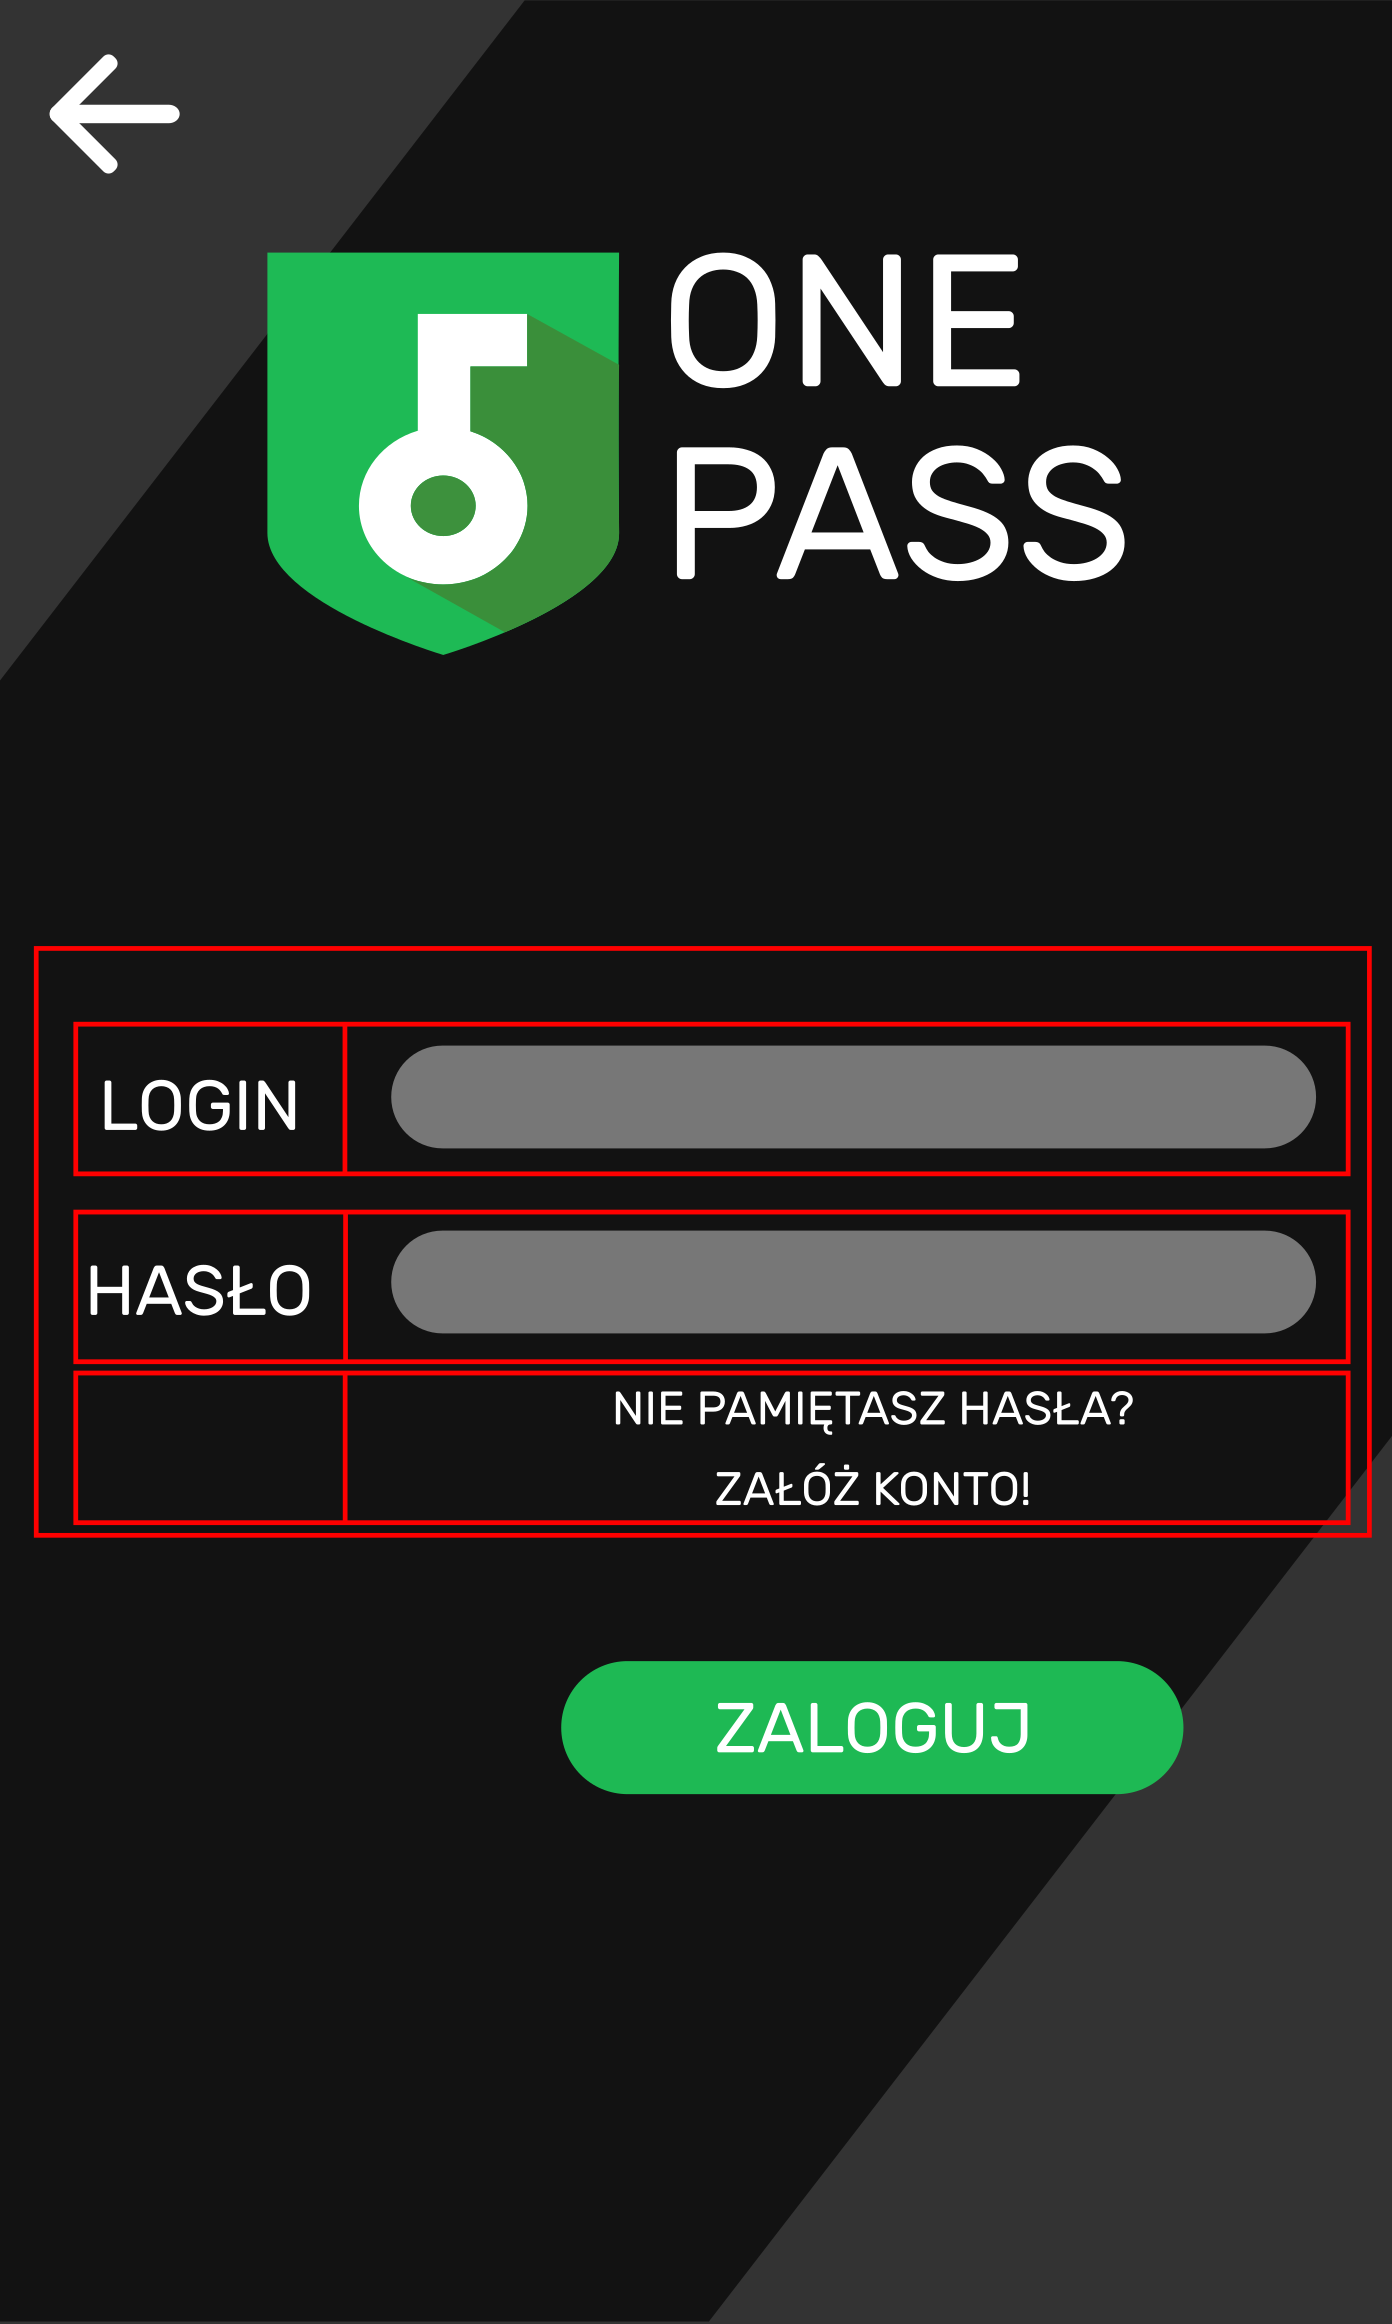
\includegraphics[height=1\textwidth]{img/ekran_logowania.png}
    \caption{Ekran logowania}
    \label{fig:logowanie}
\end{figure}

\begin{figure}[H]
    \centering
    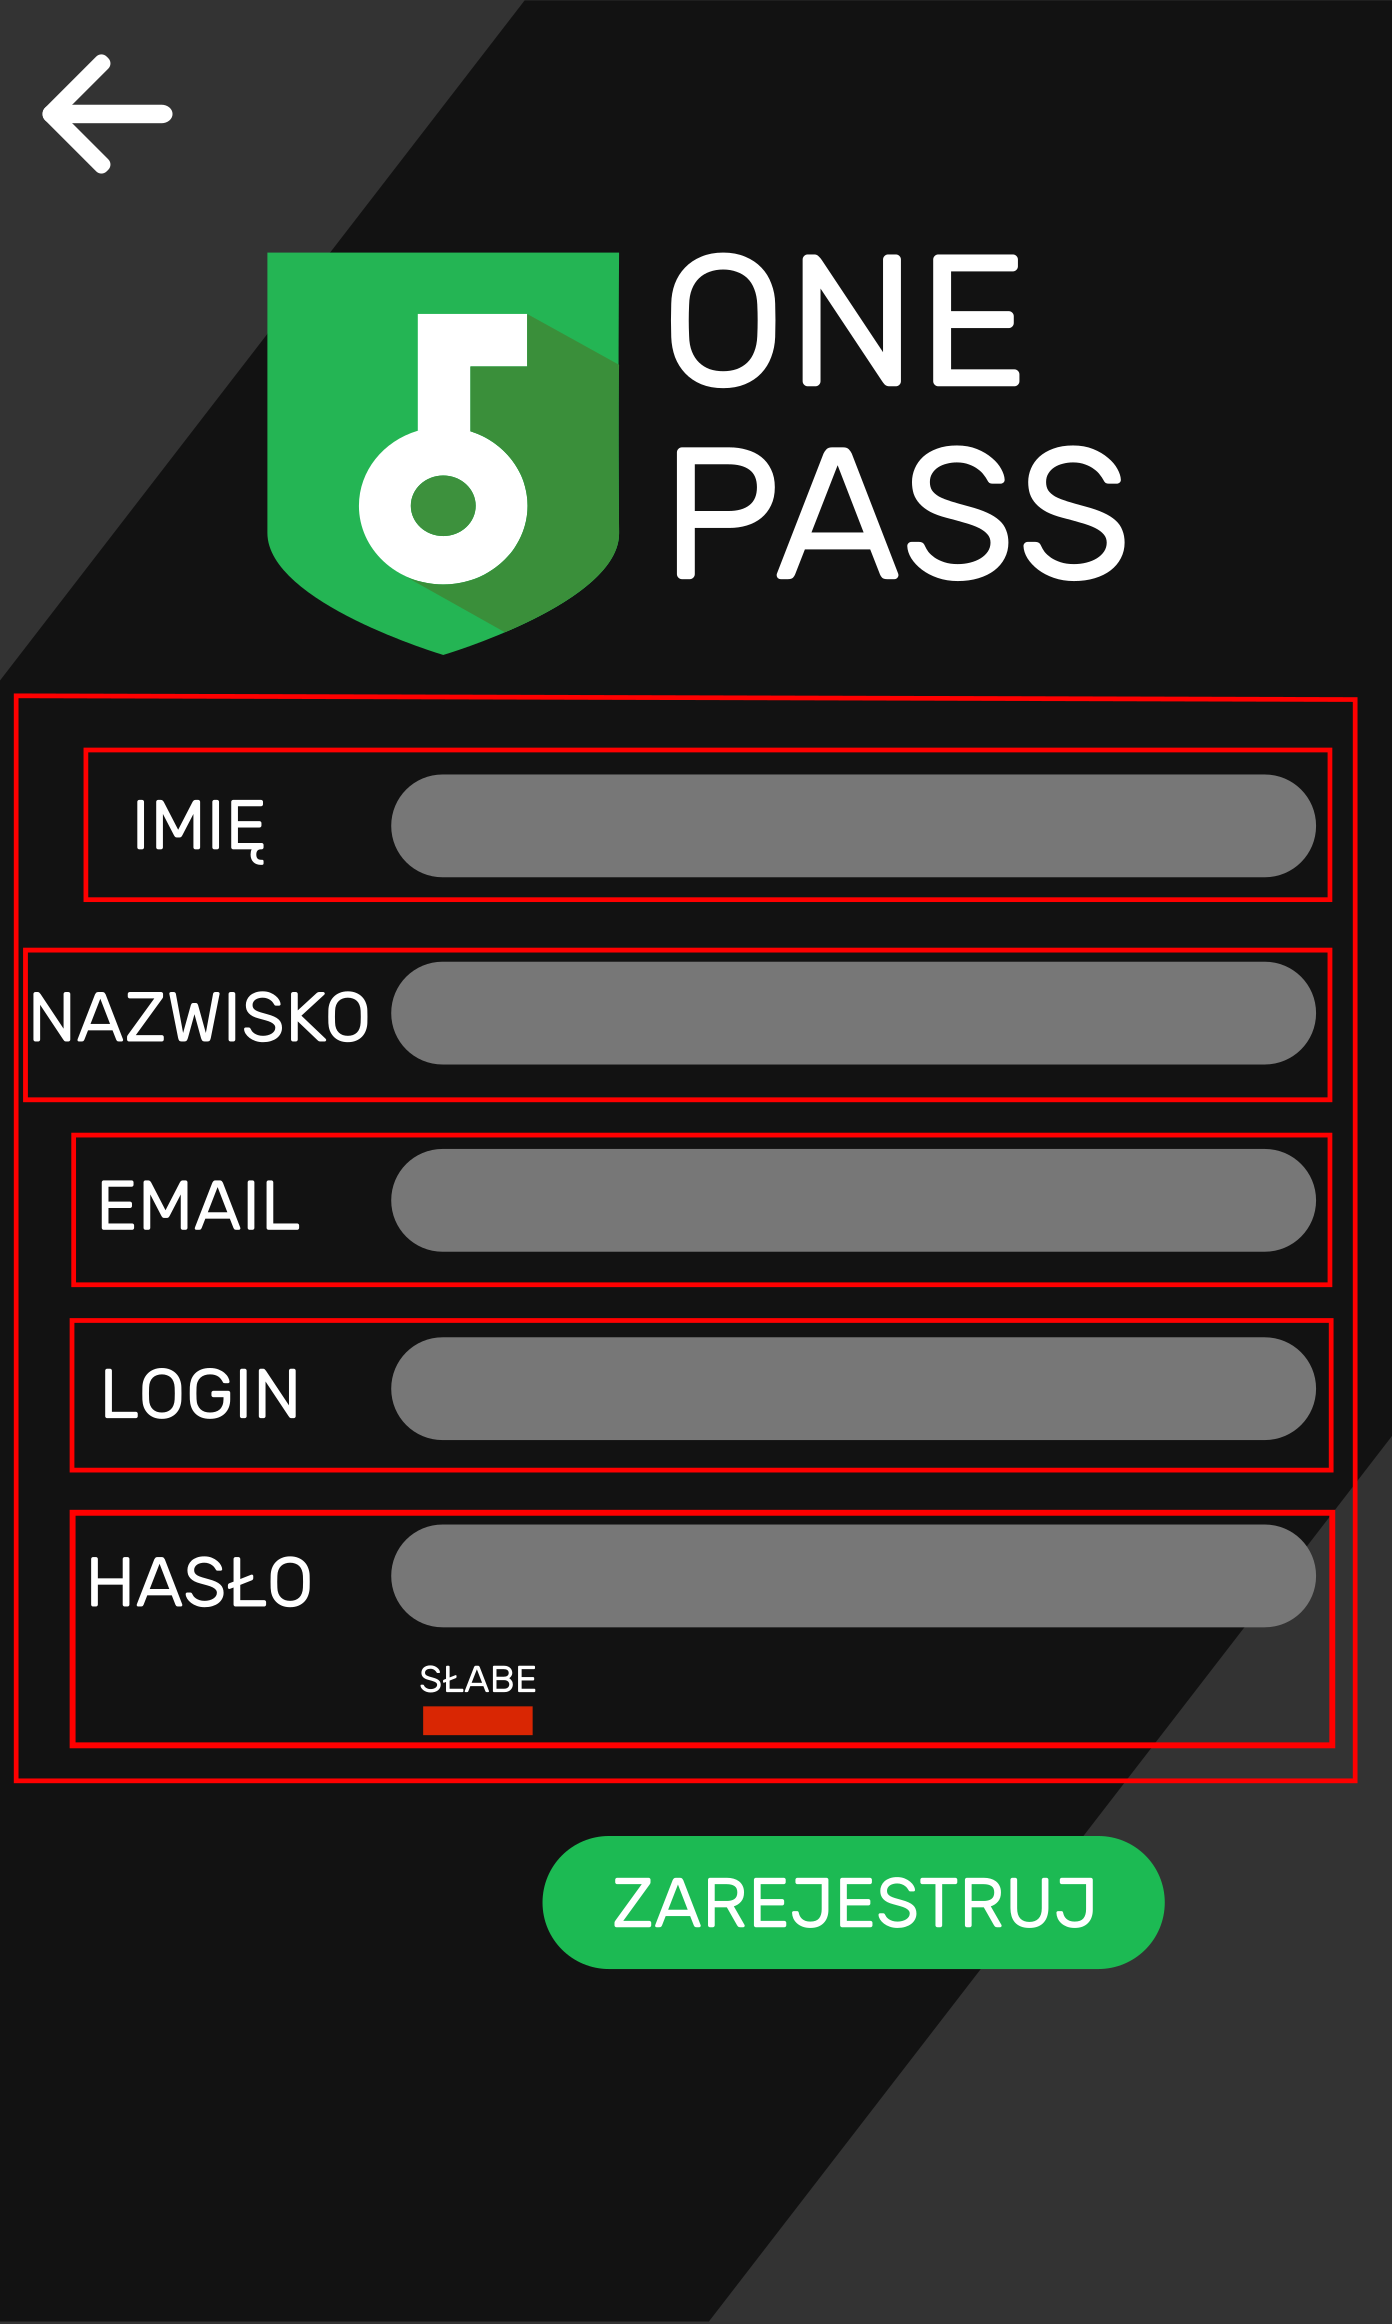
\includegraphics[height=1\textwidth]{img/ekran_rej.png}
    \caption{Ekran rejestracji}
    \label{fig:rejestracja}
\end{figure}

\begin{figure}[H]
    \centering
    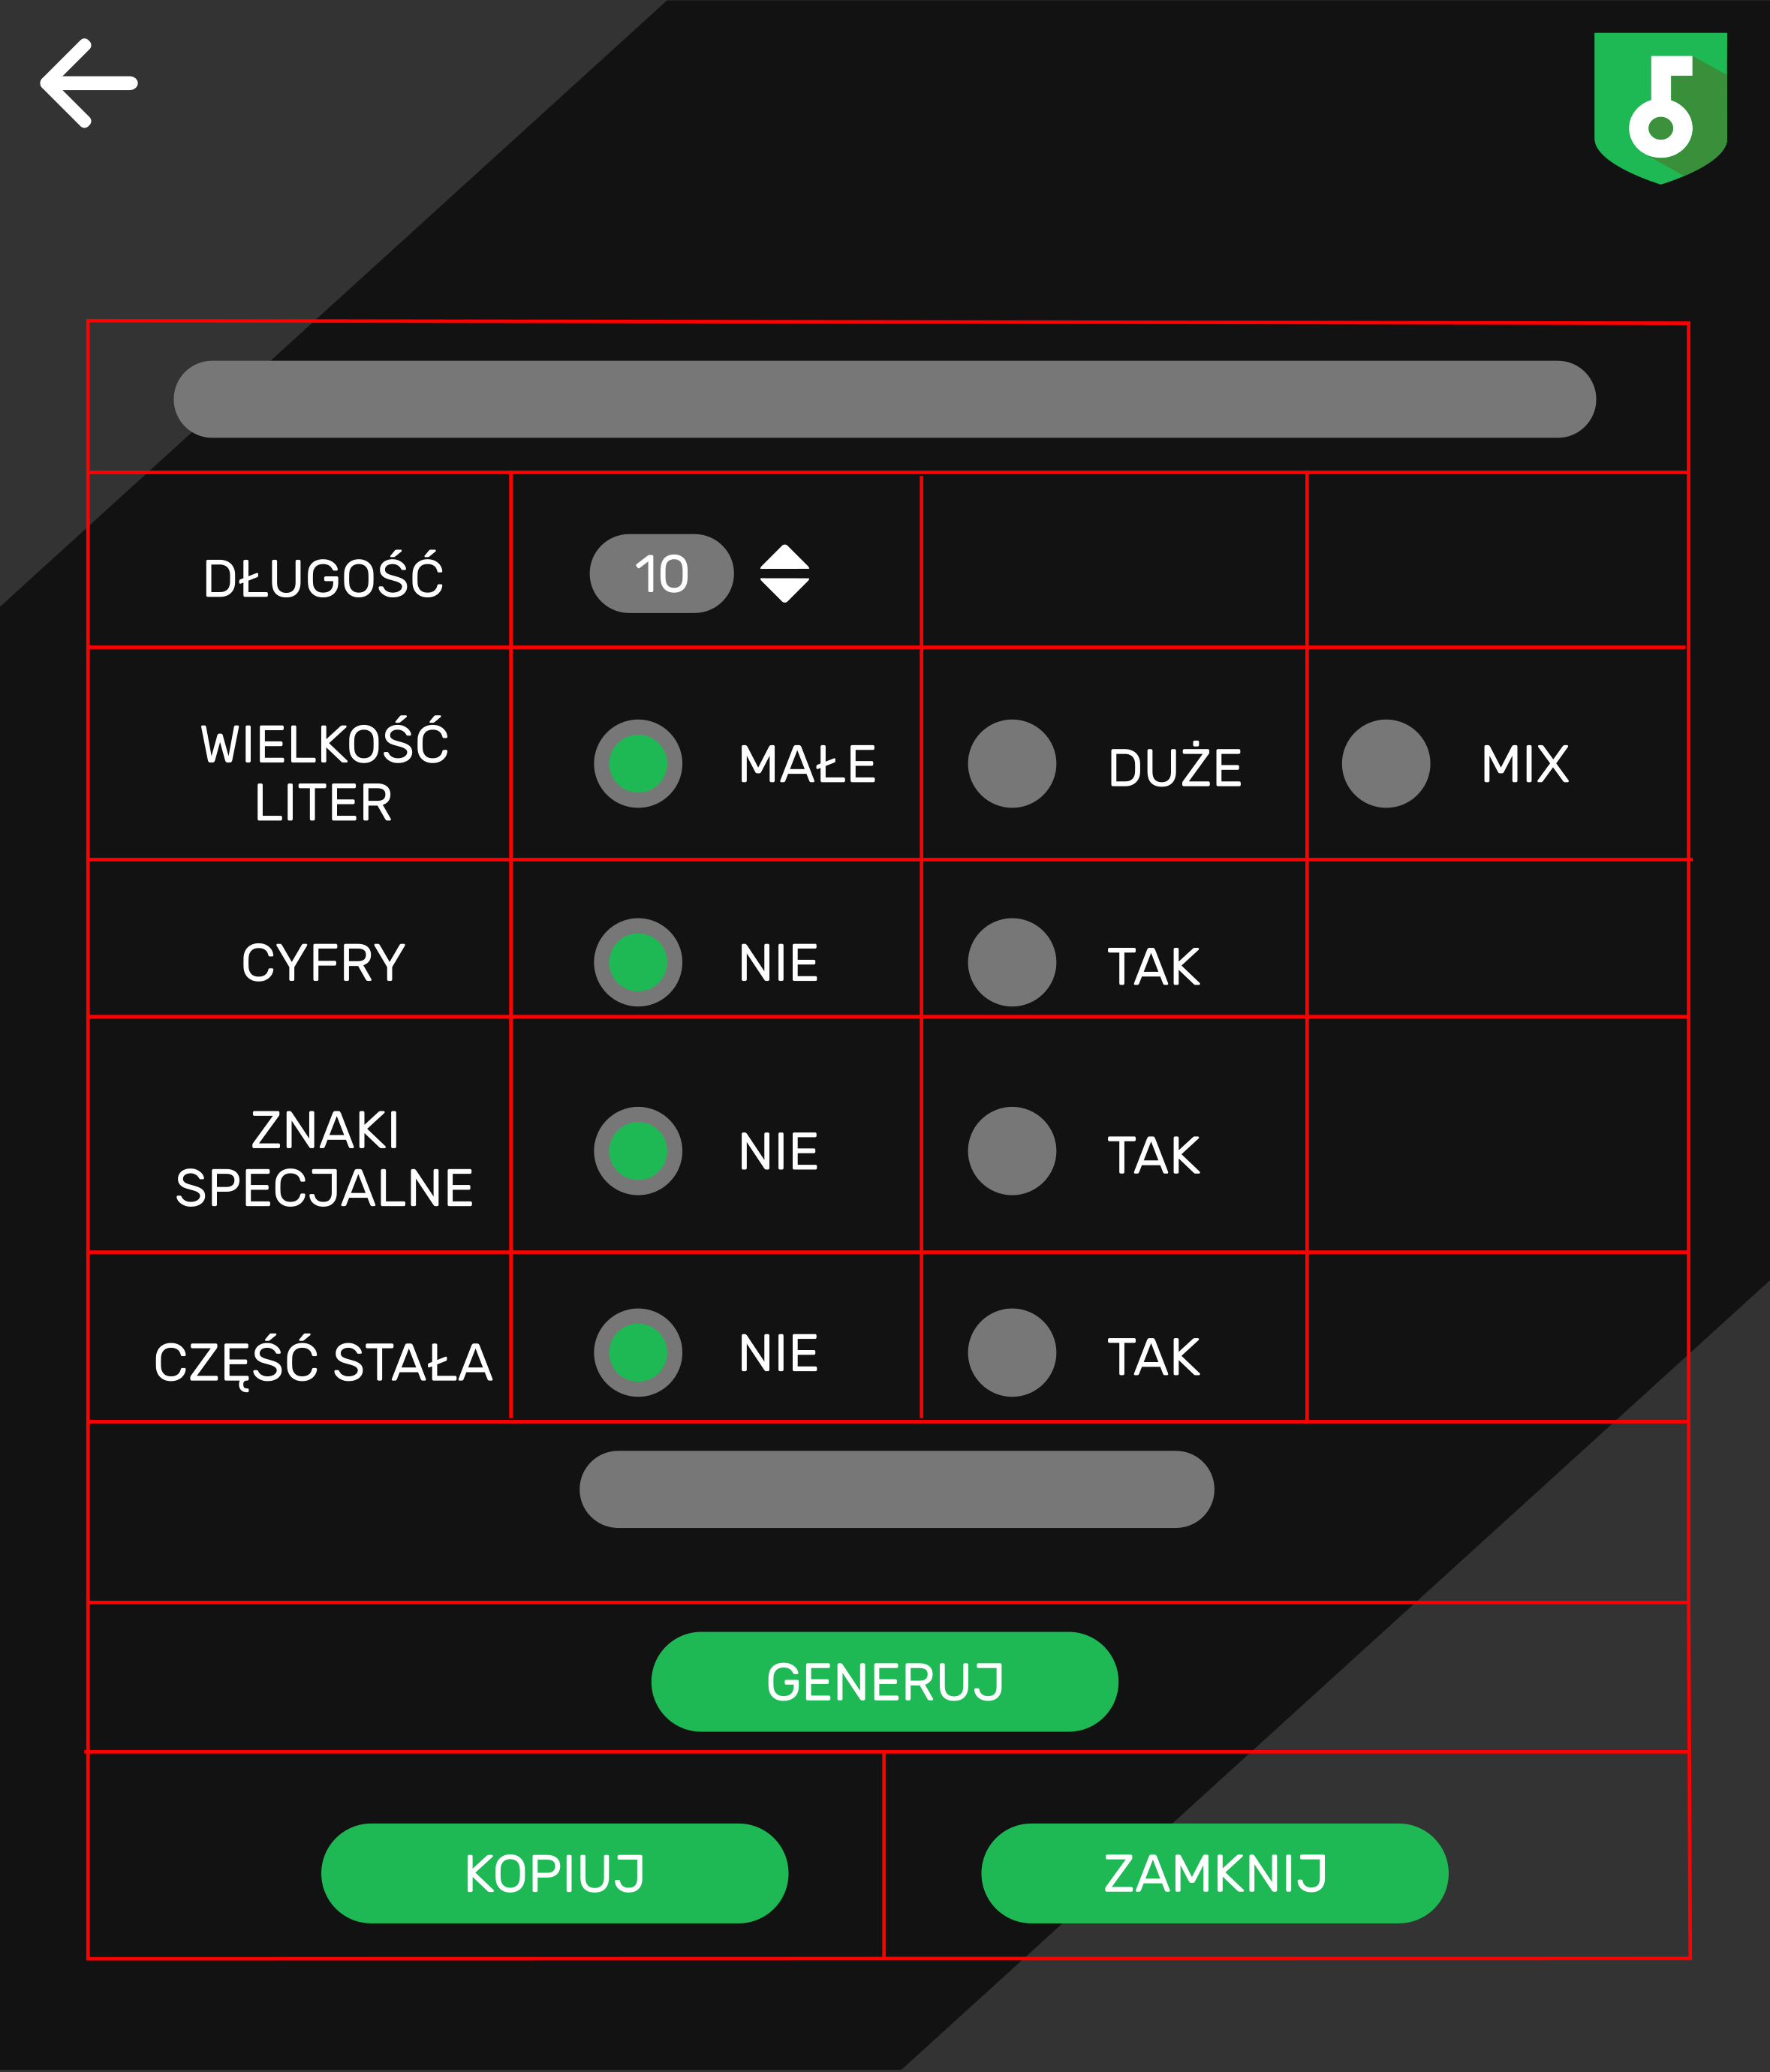
\includegraphics[height=1\textwidth]{img/ekran_generacji.png}
    \caption{Ekran generowania haseł}
    \label{fig:profil}
\end{figure}

\begin{figure}[H]
    \centering
    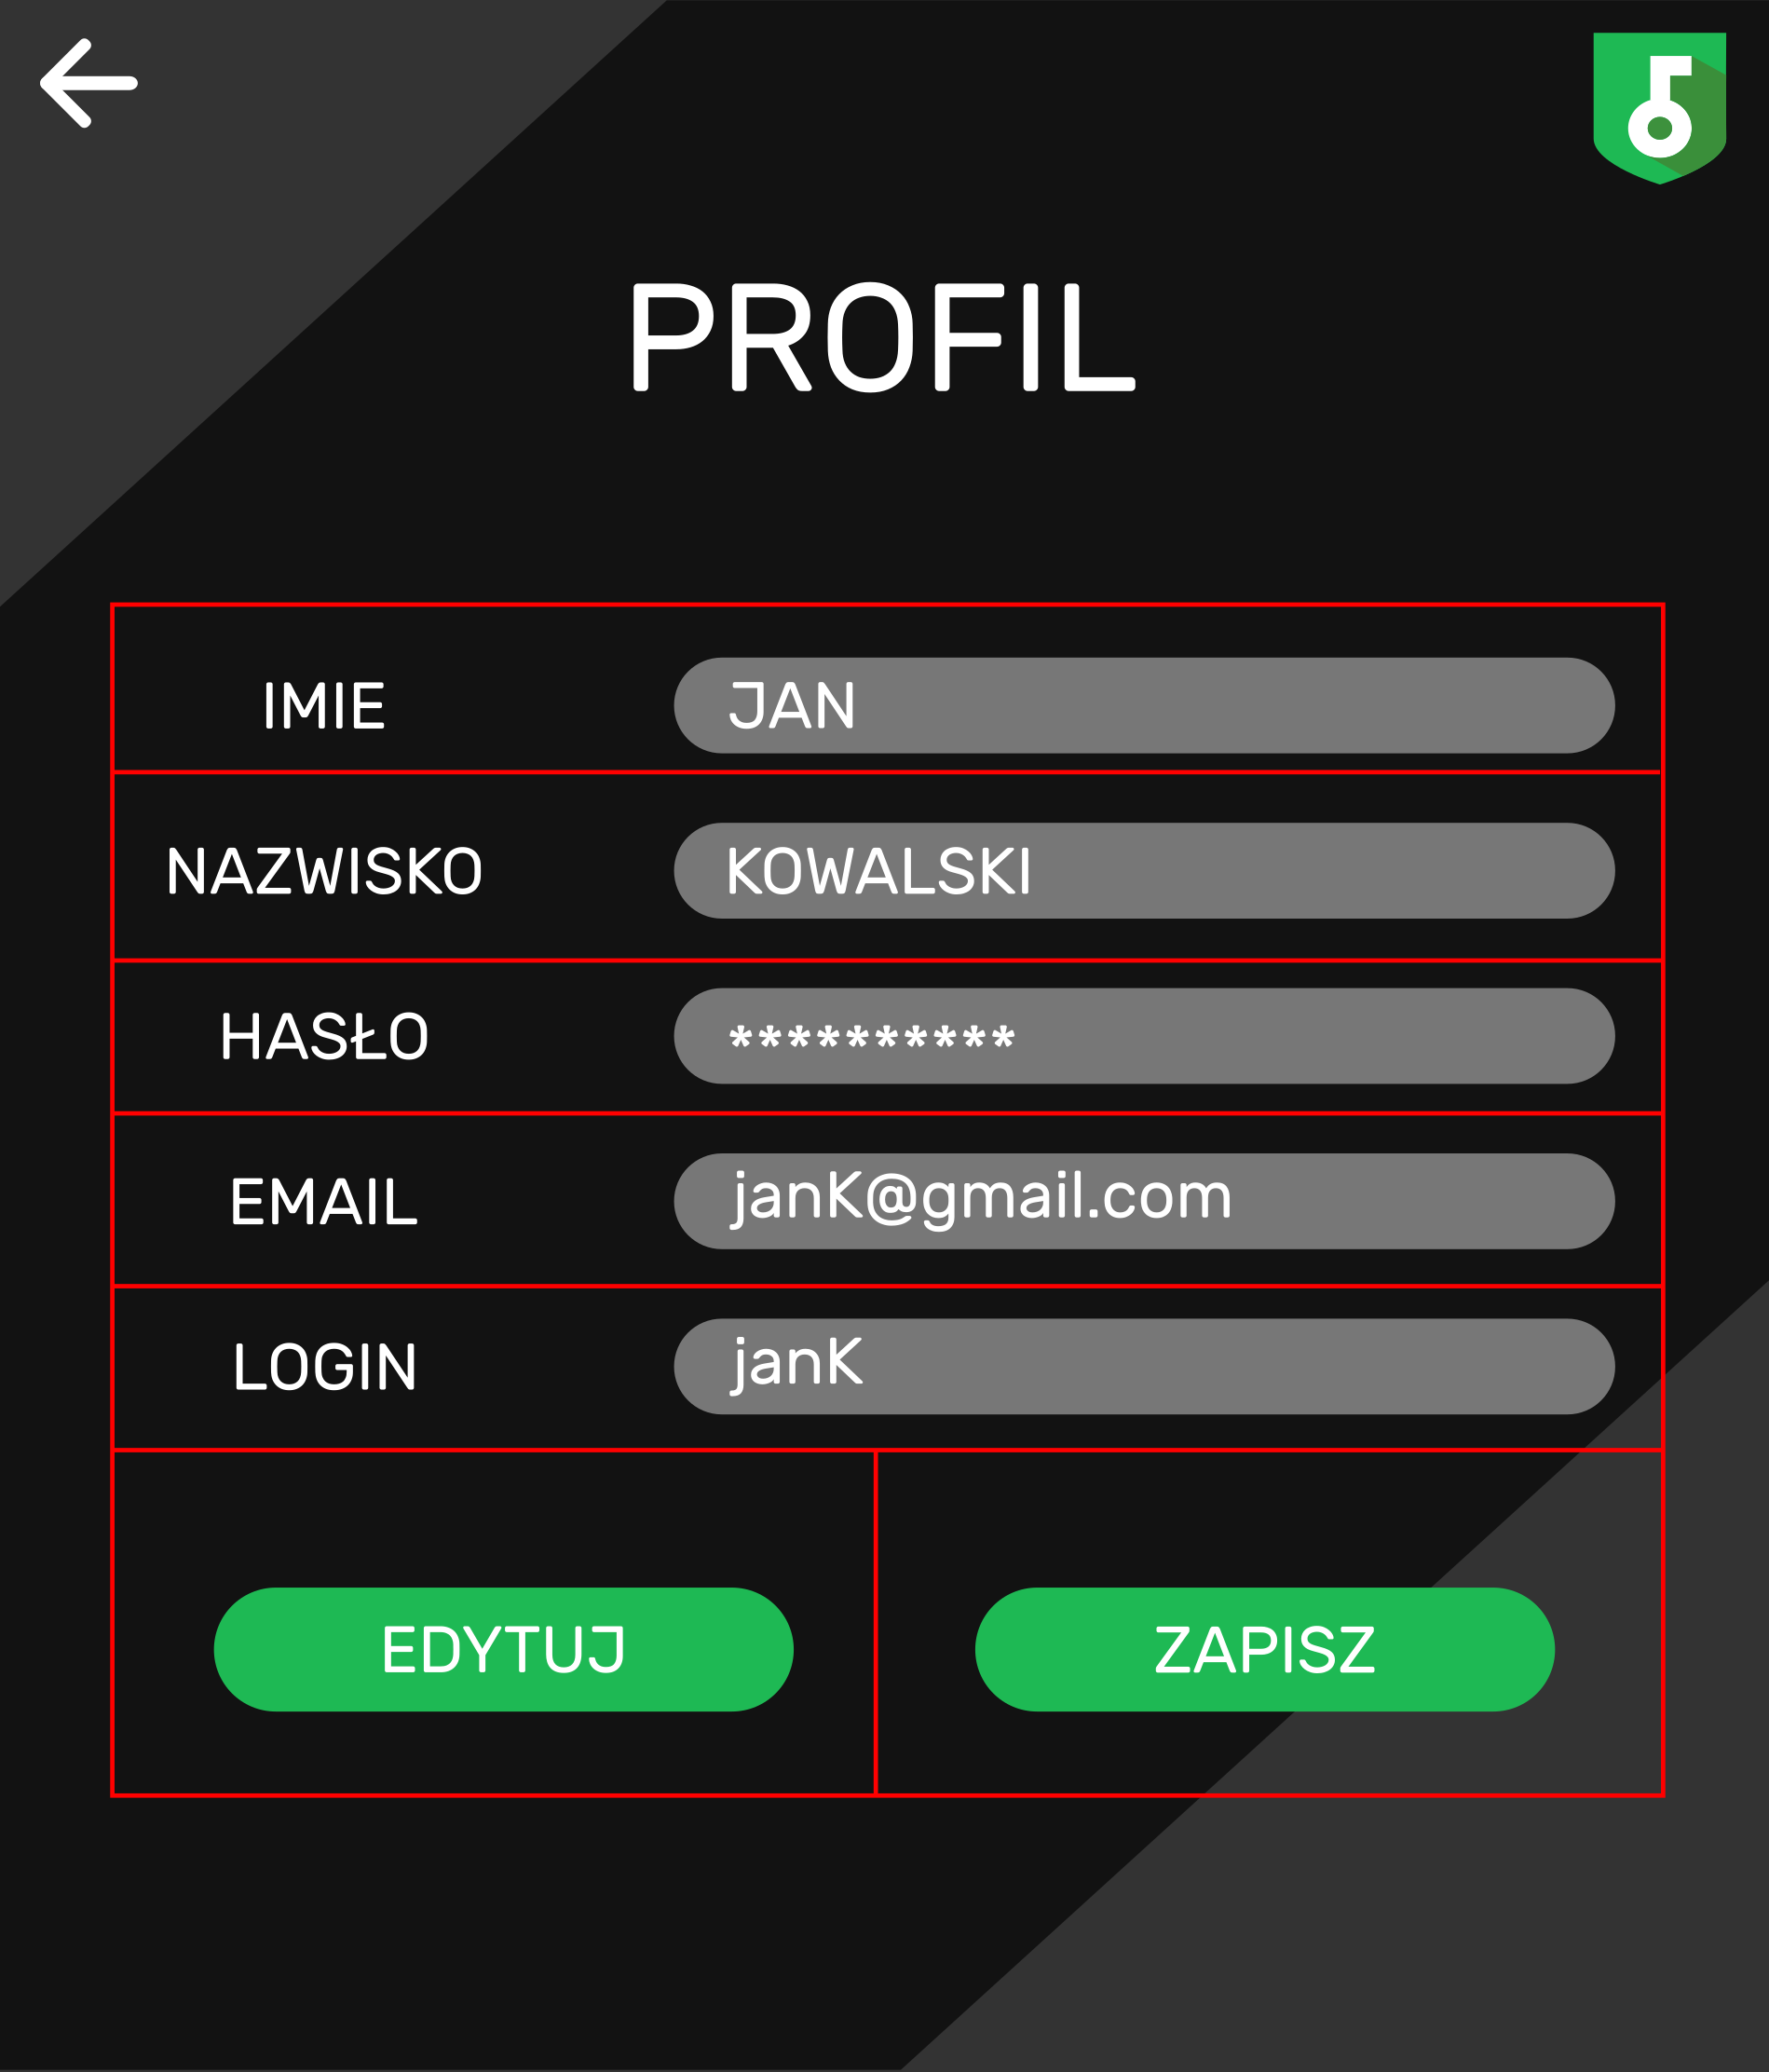
\includegraphics[height=1\textwidth]{img/ekran_profilu.png}
    \caption{Ekran informacji o profilu}
    \label{fig:profil}
\end{figure}

\begin{figure}[H]
    \centering
    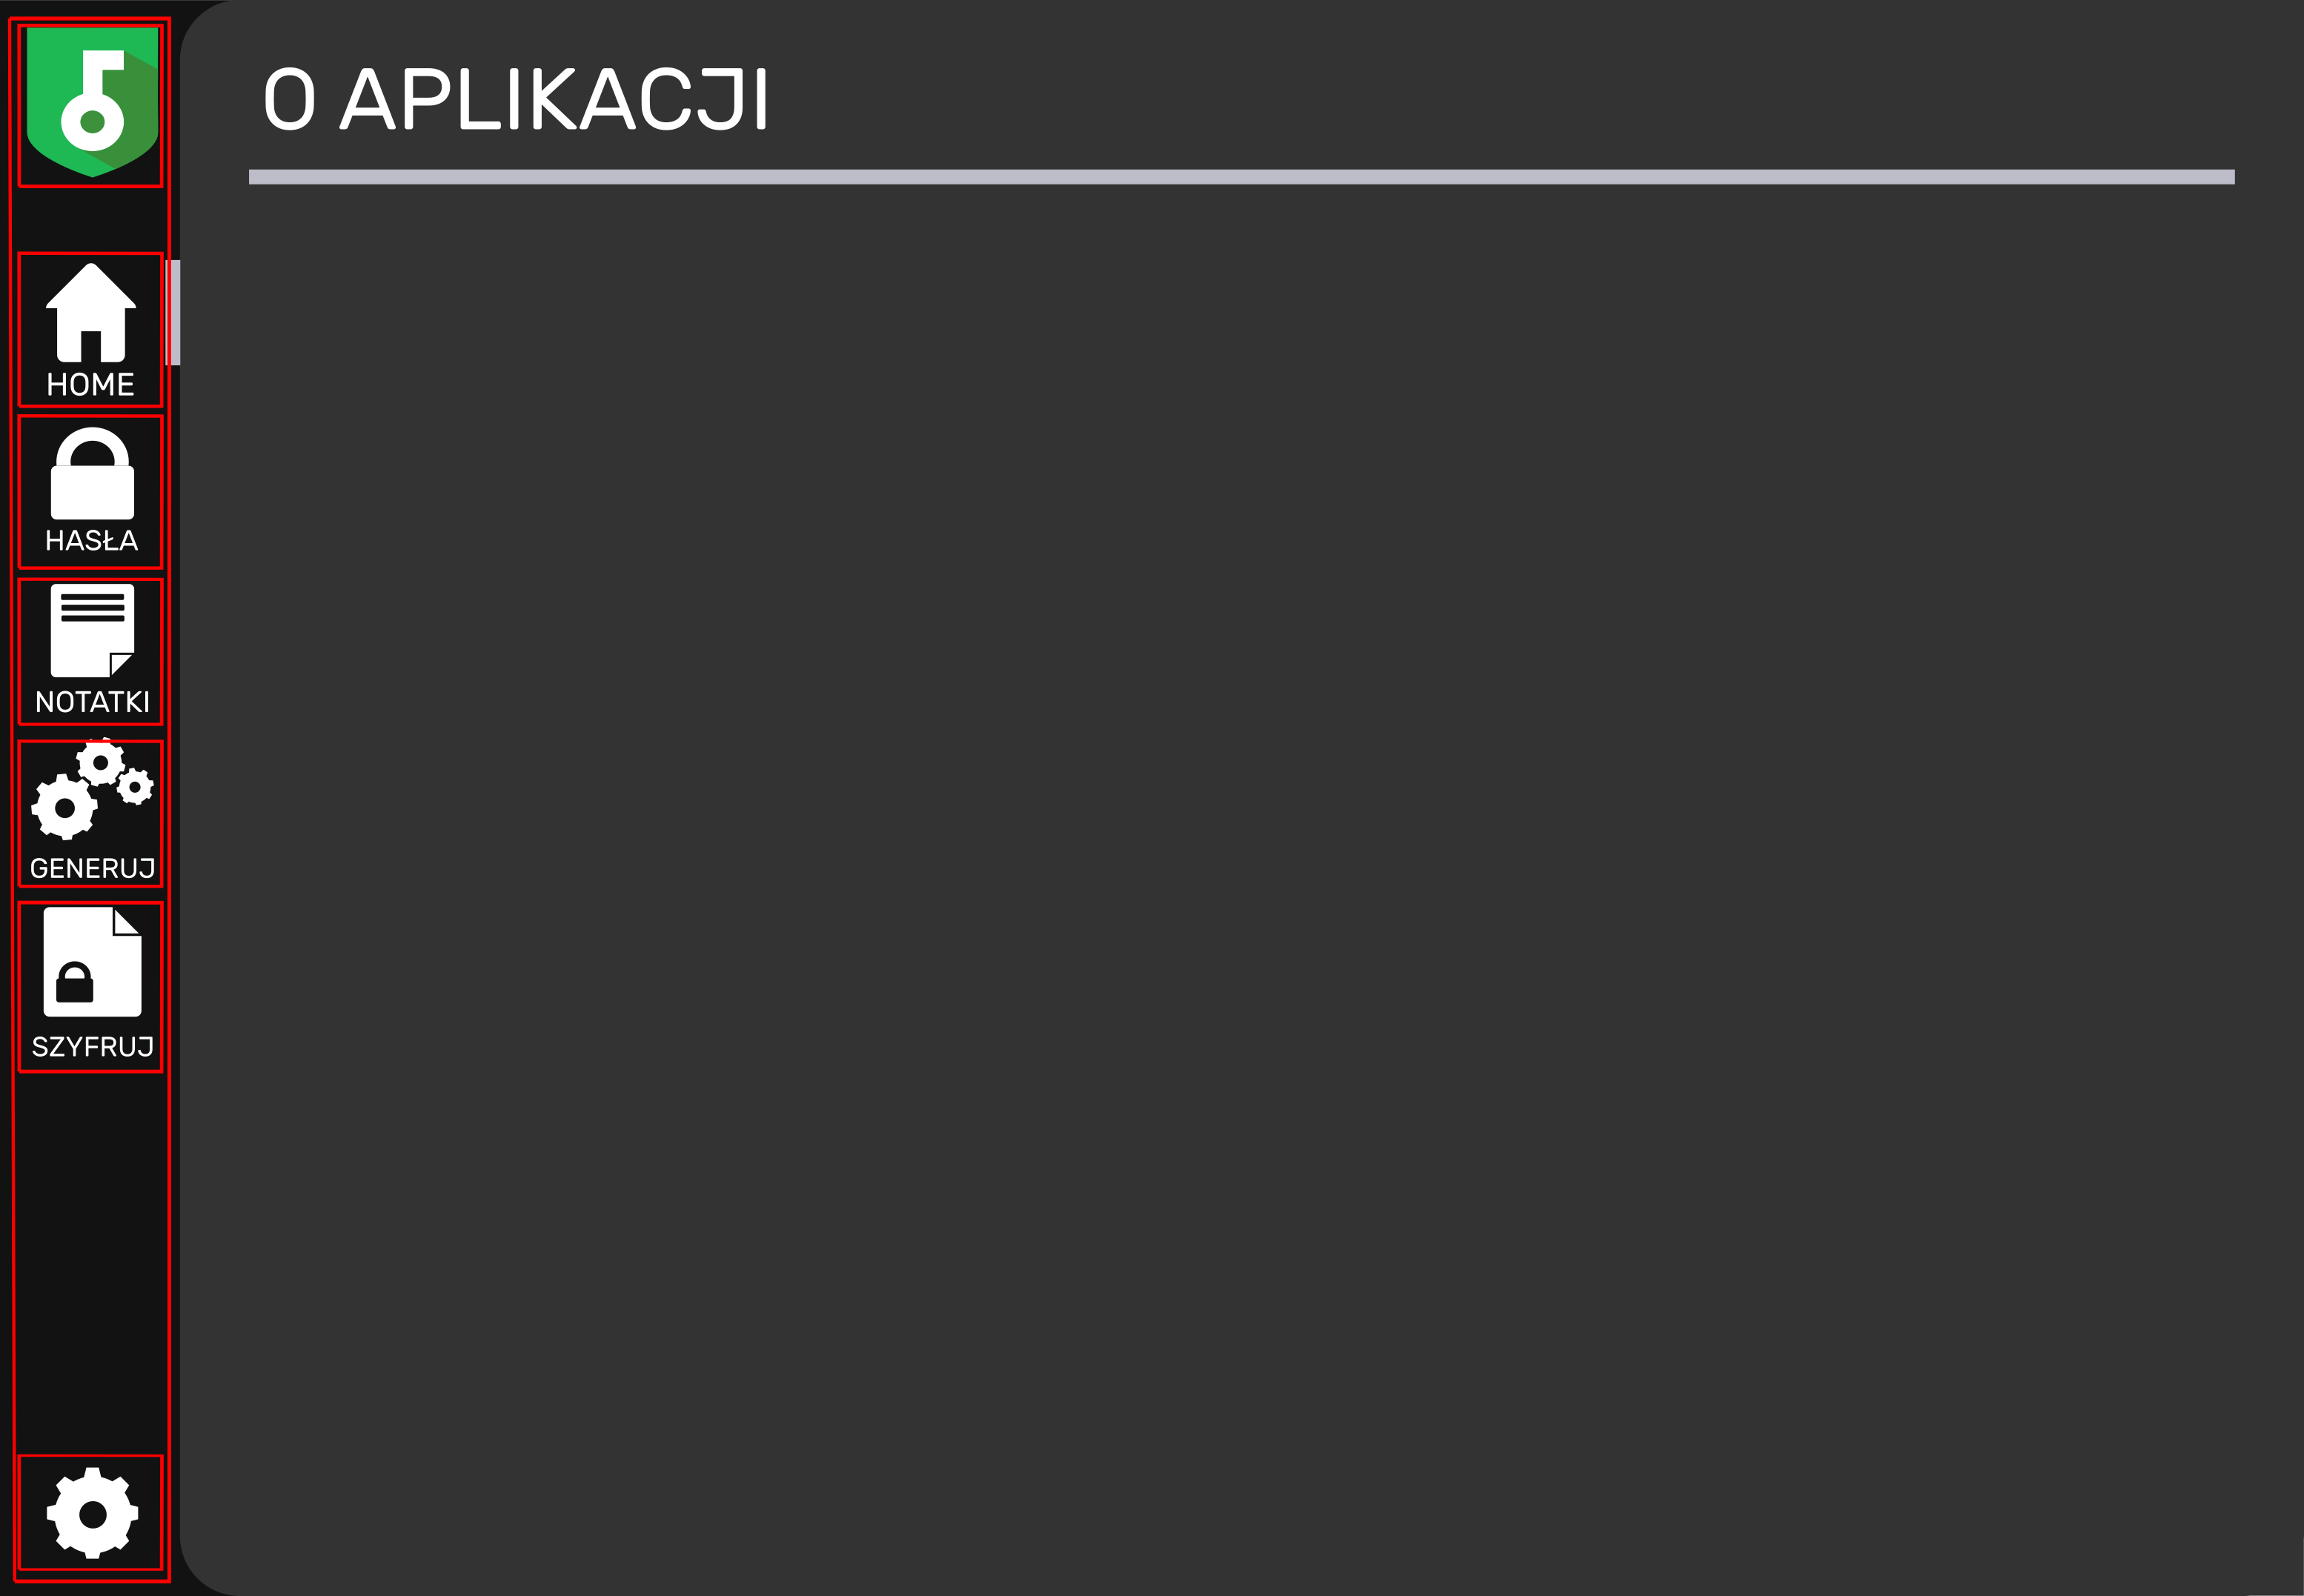
\includegraphics[height=1\textwidth]{img/ekarn_oapp.png}
    \caption{Ekran o aplikacji}
    \label{fig:oApp}
\end{figure}

\begin{figure}[H]
    \centering
    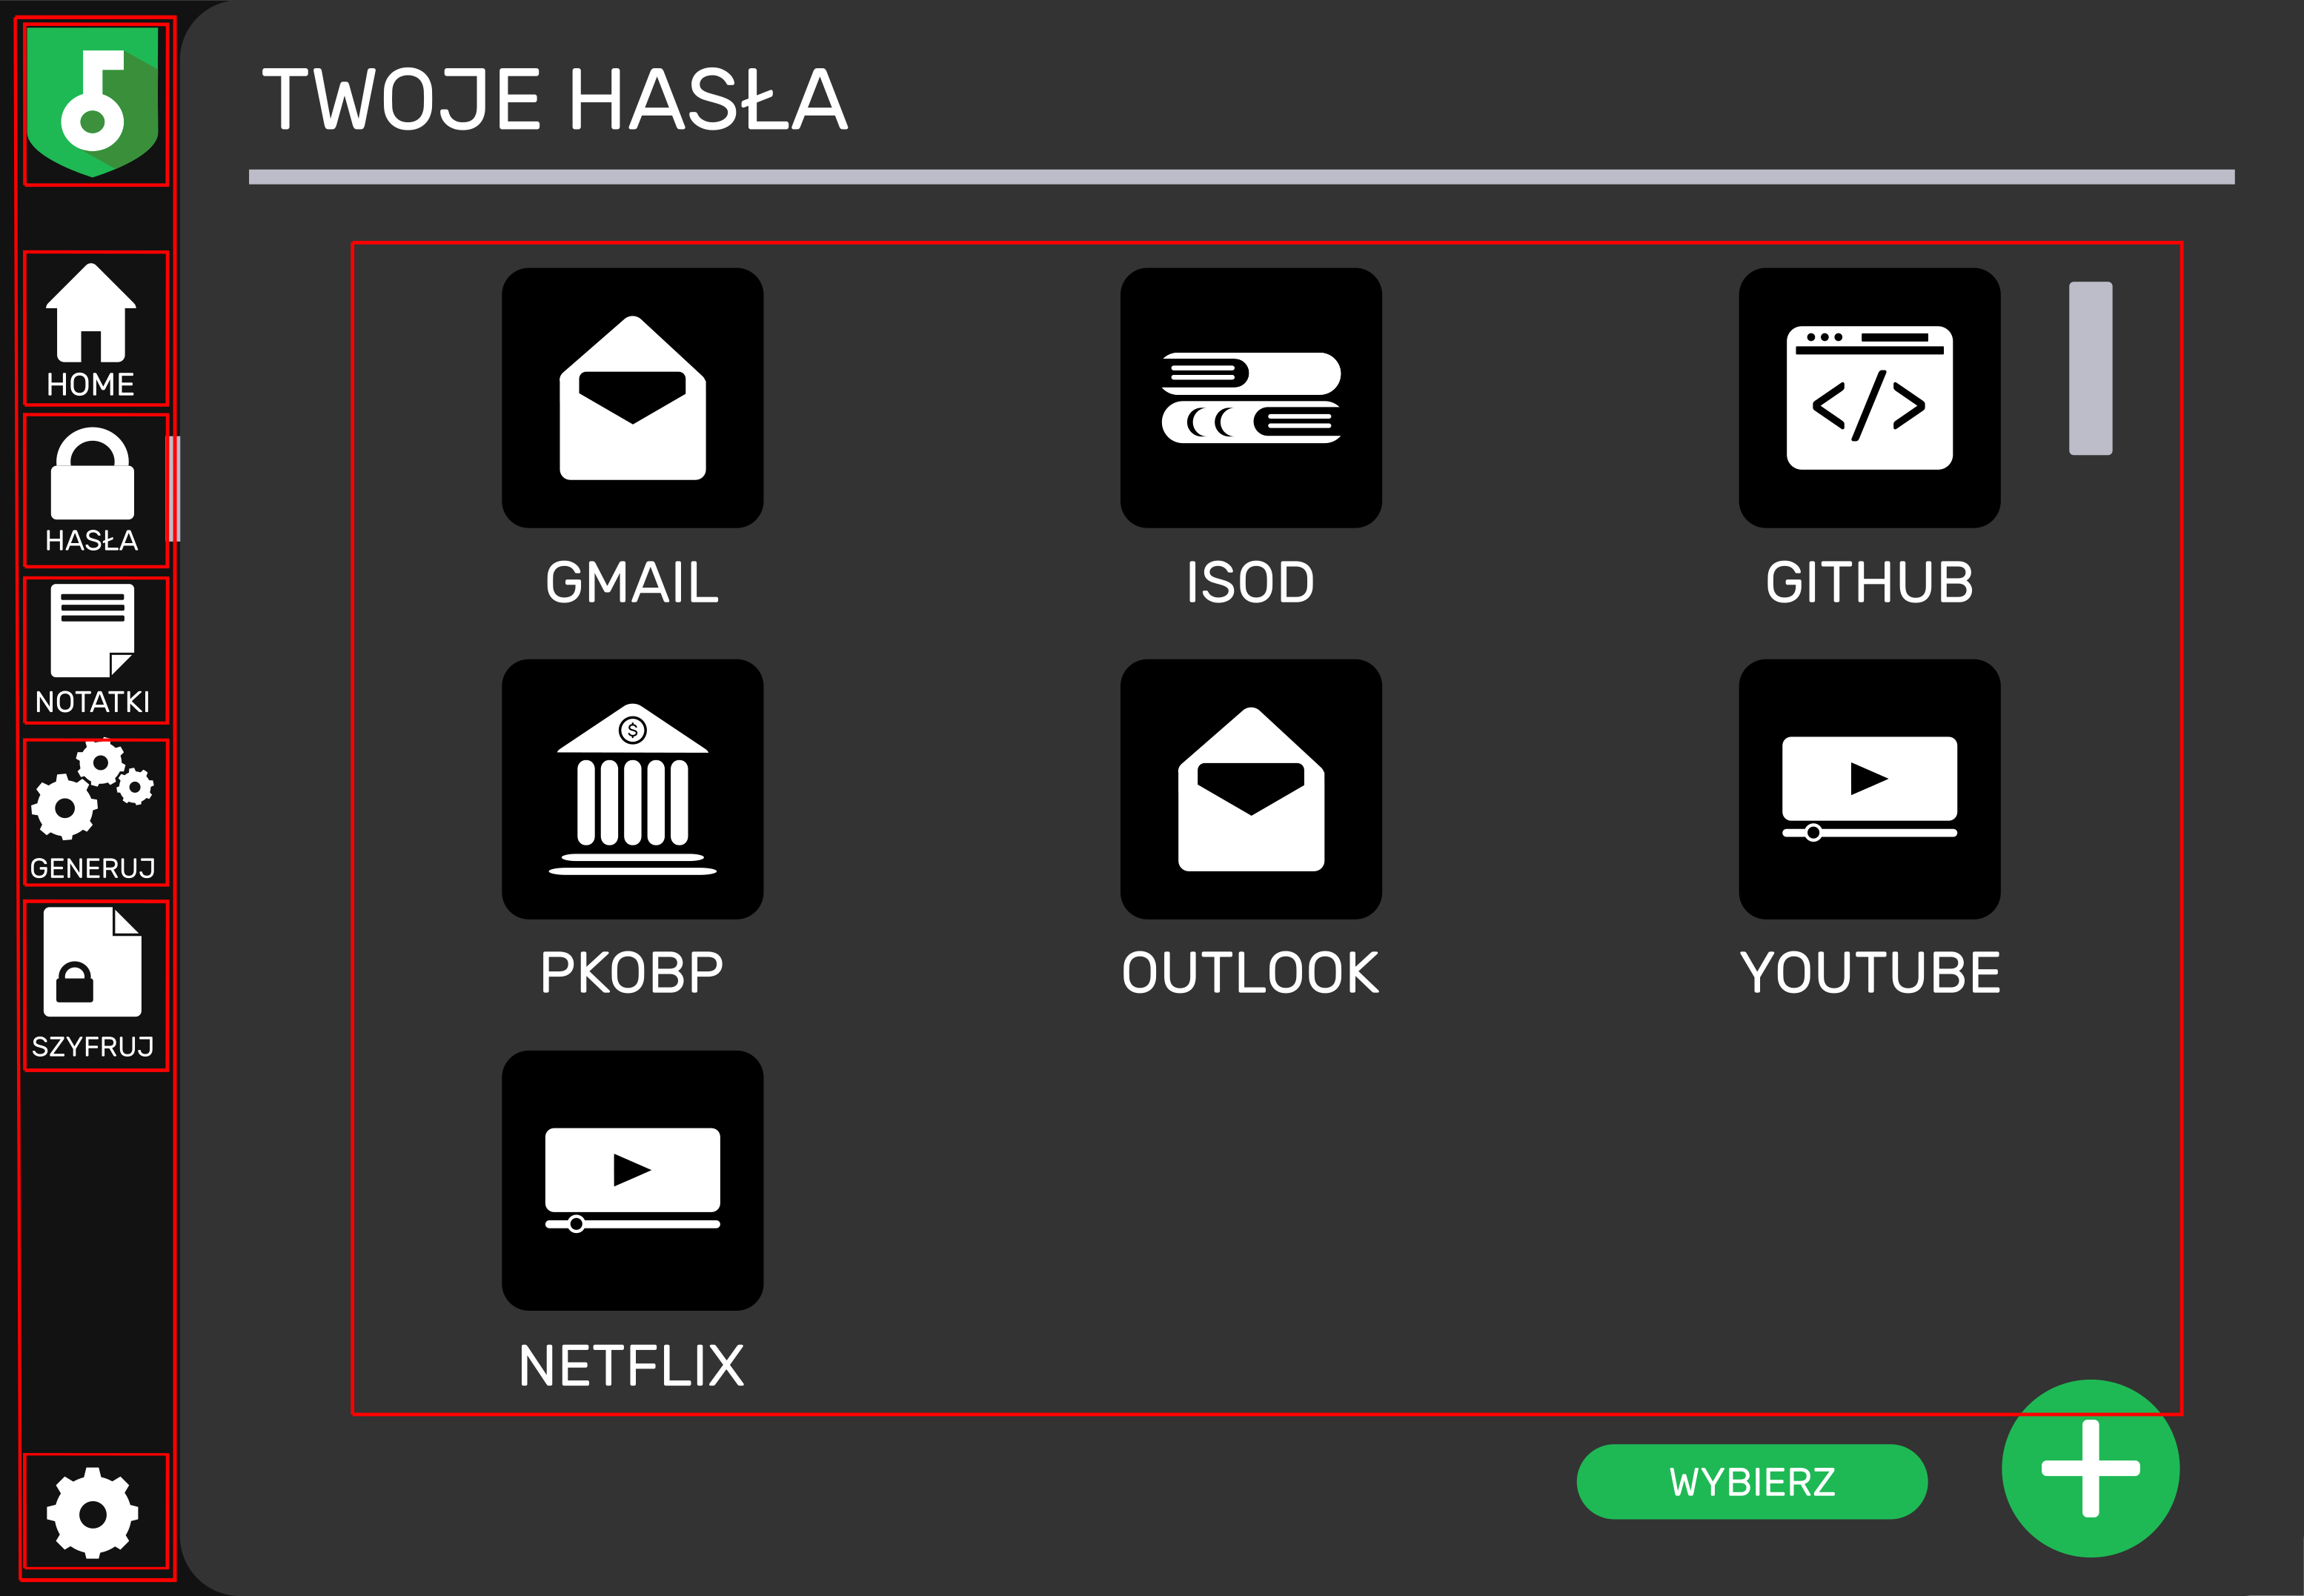
\includegraphics[width=1\textwidth]{img/ekran_hasel.png}
    \caption{Ekran haseł}
    \label{fig:hasla}
\end{figure}

\begin{figure}[H]
    \centering
    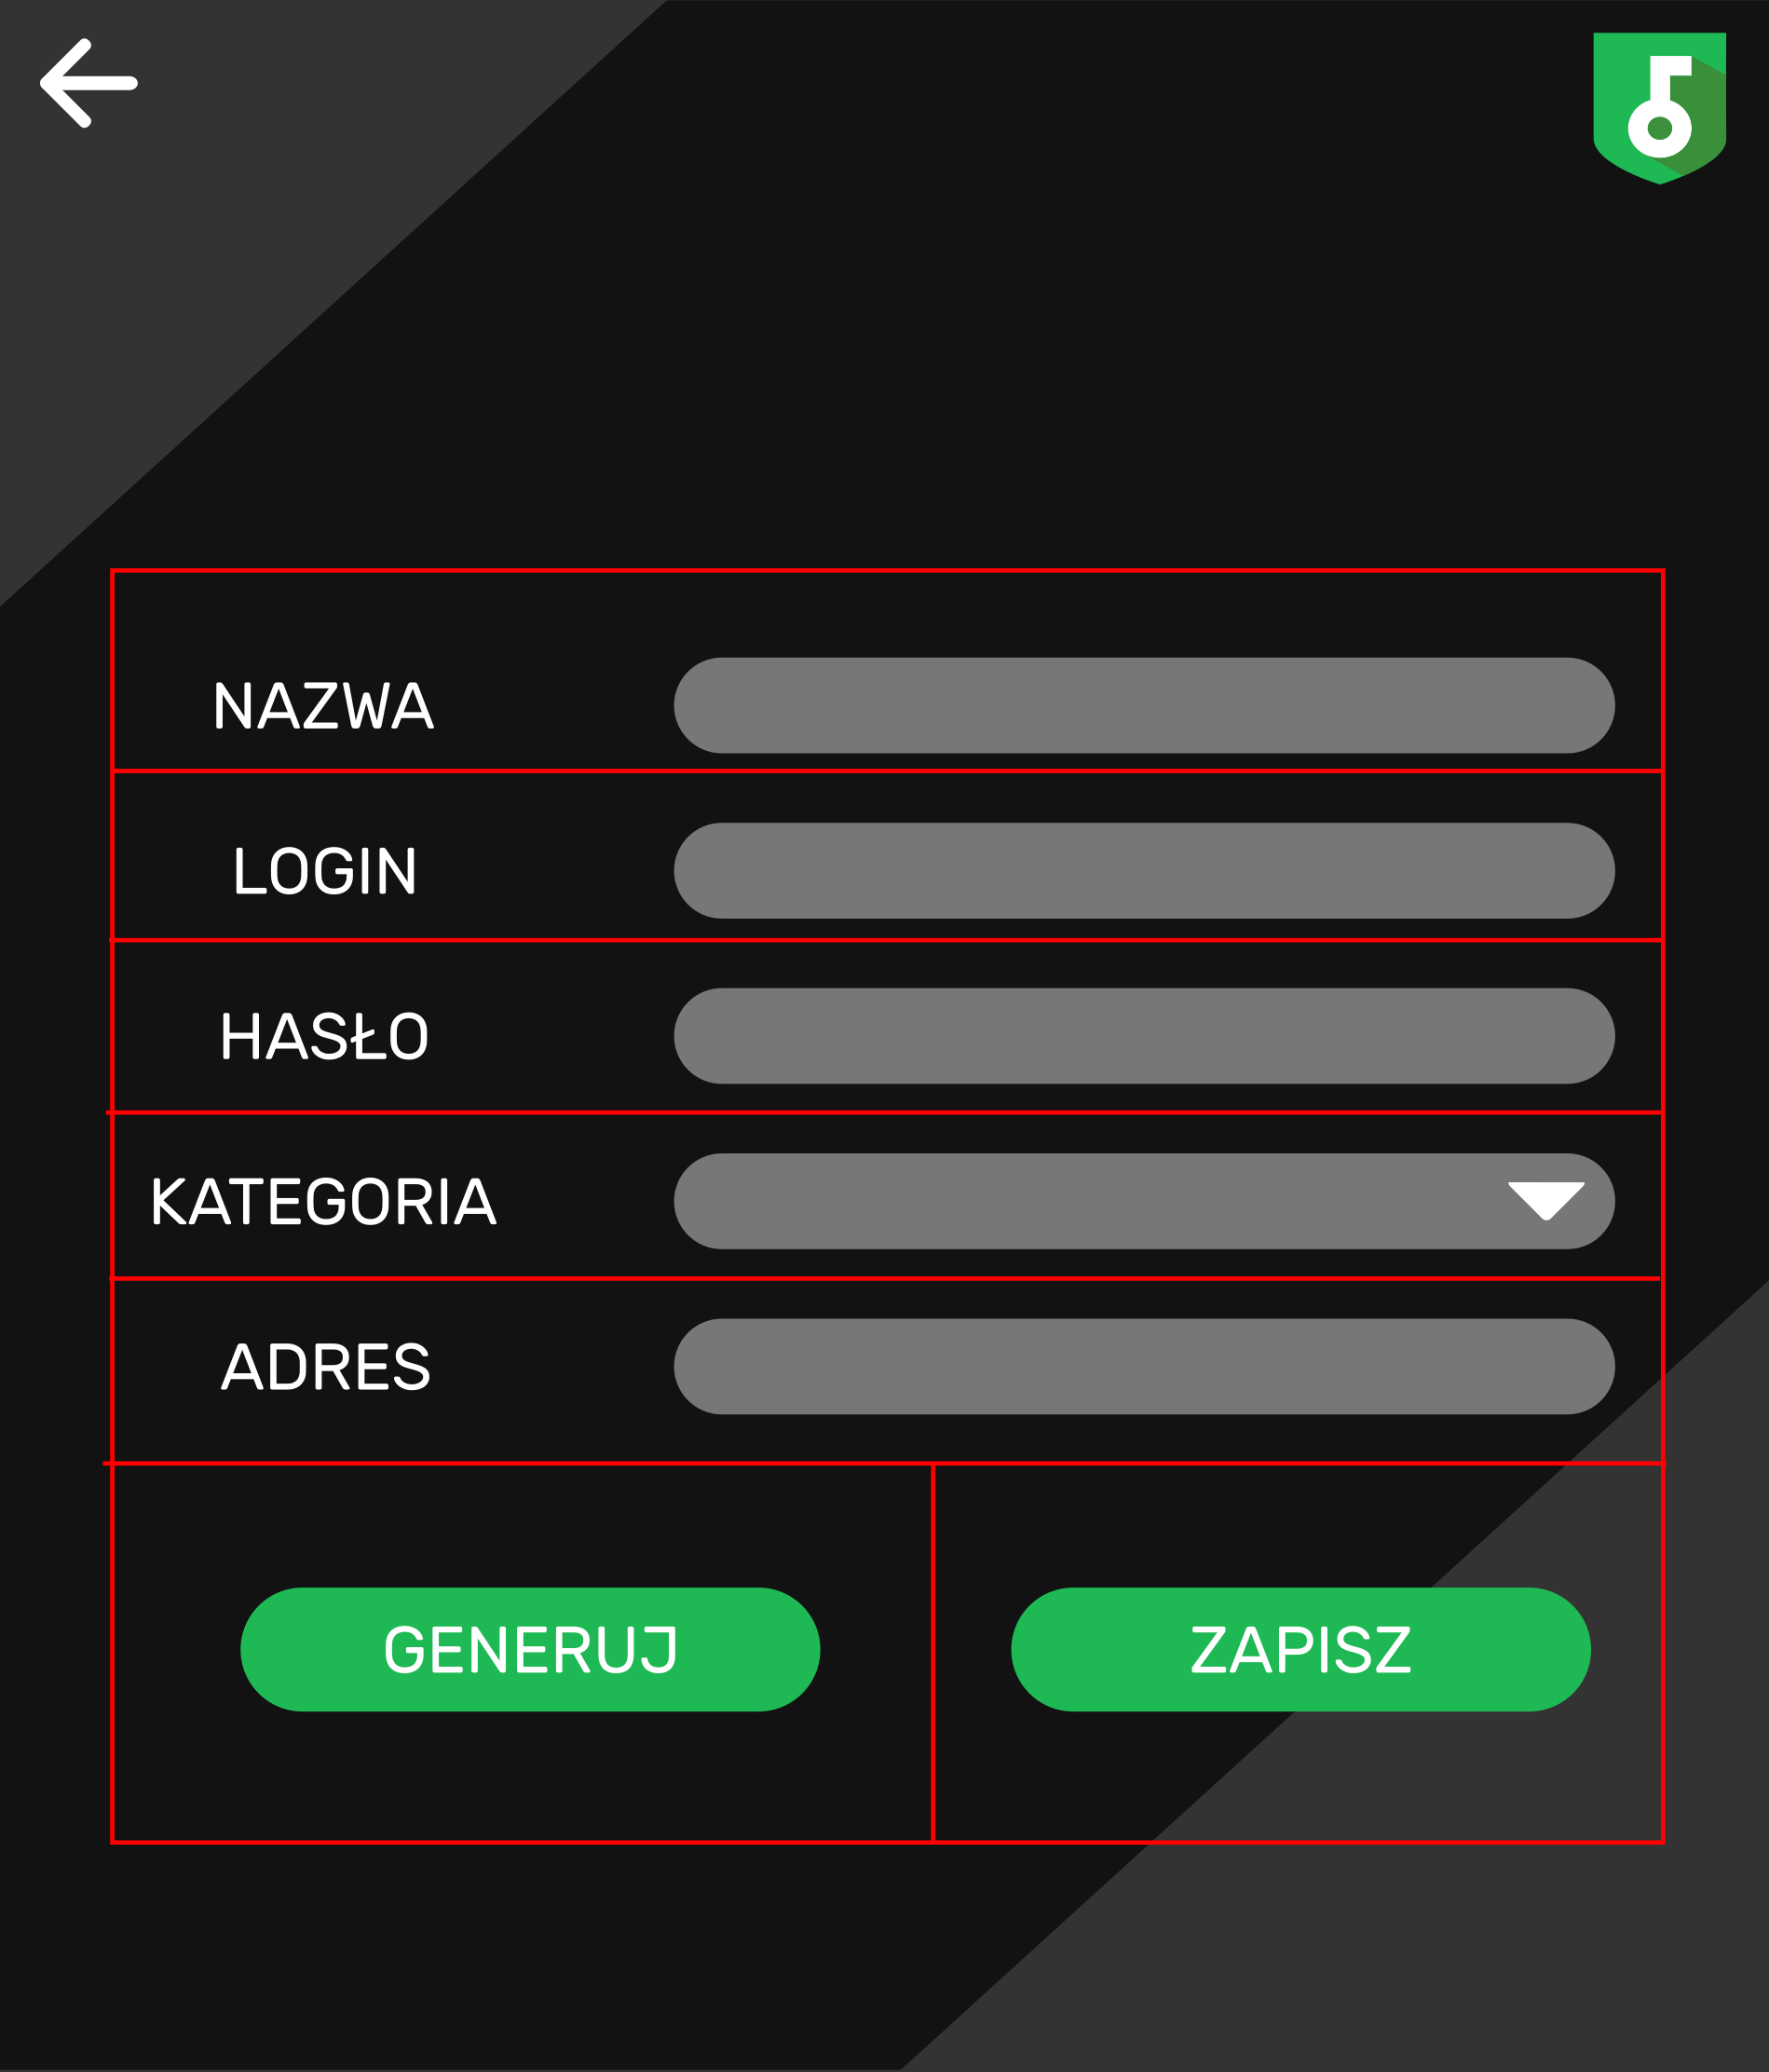
\includegraphics[height=1\textwidth]{img/ekran_dodania.png}
    \caption{Ekran dodawania obiektu}
    \label{fig:haslaDodanie}
\end{figure}

\begin{figure}[H]
    \centering
    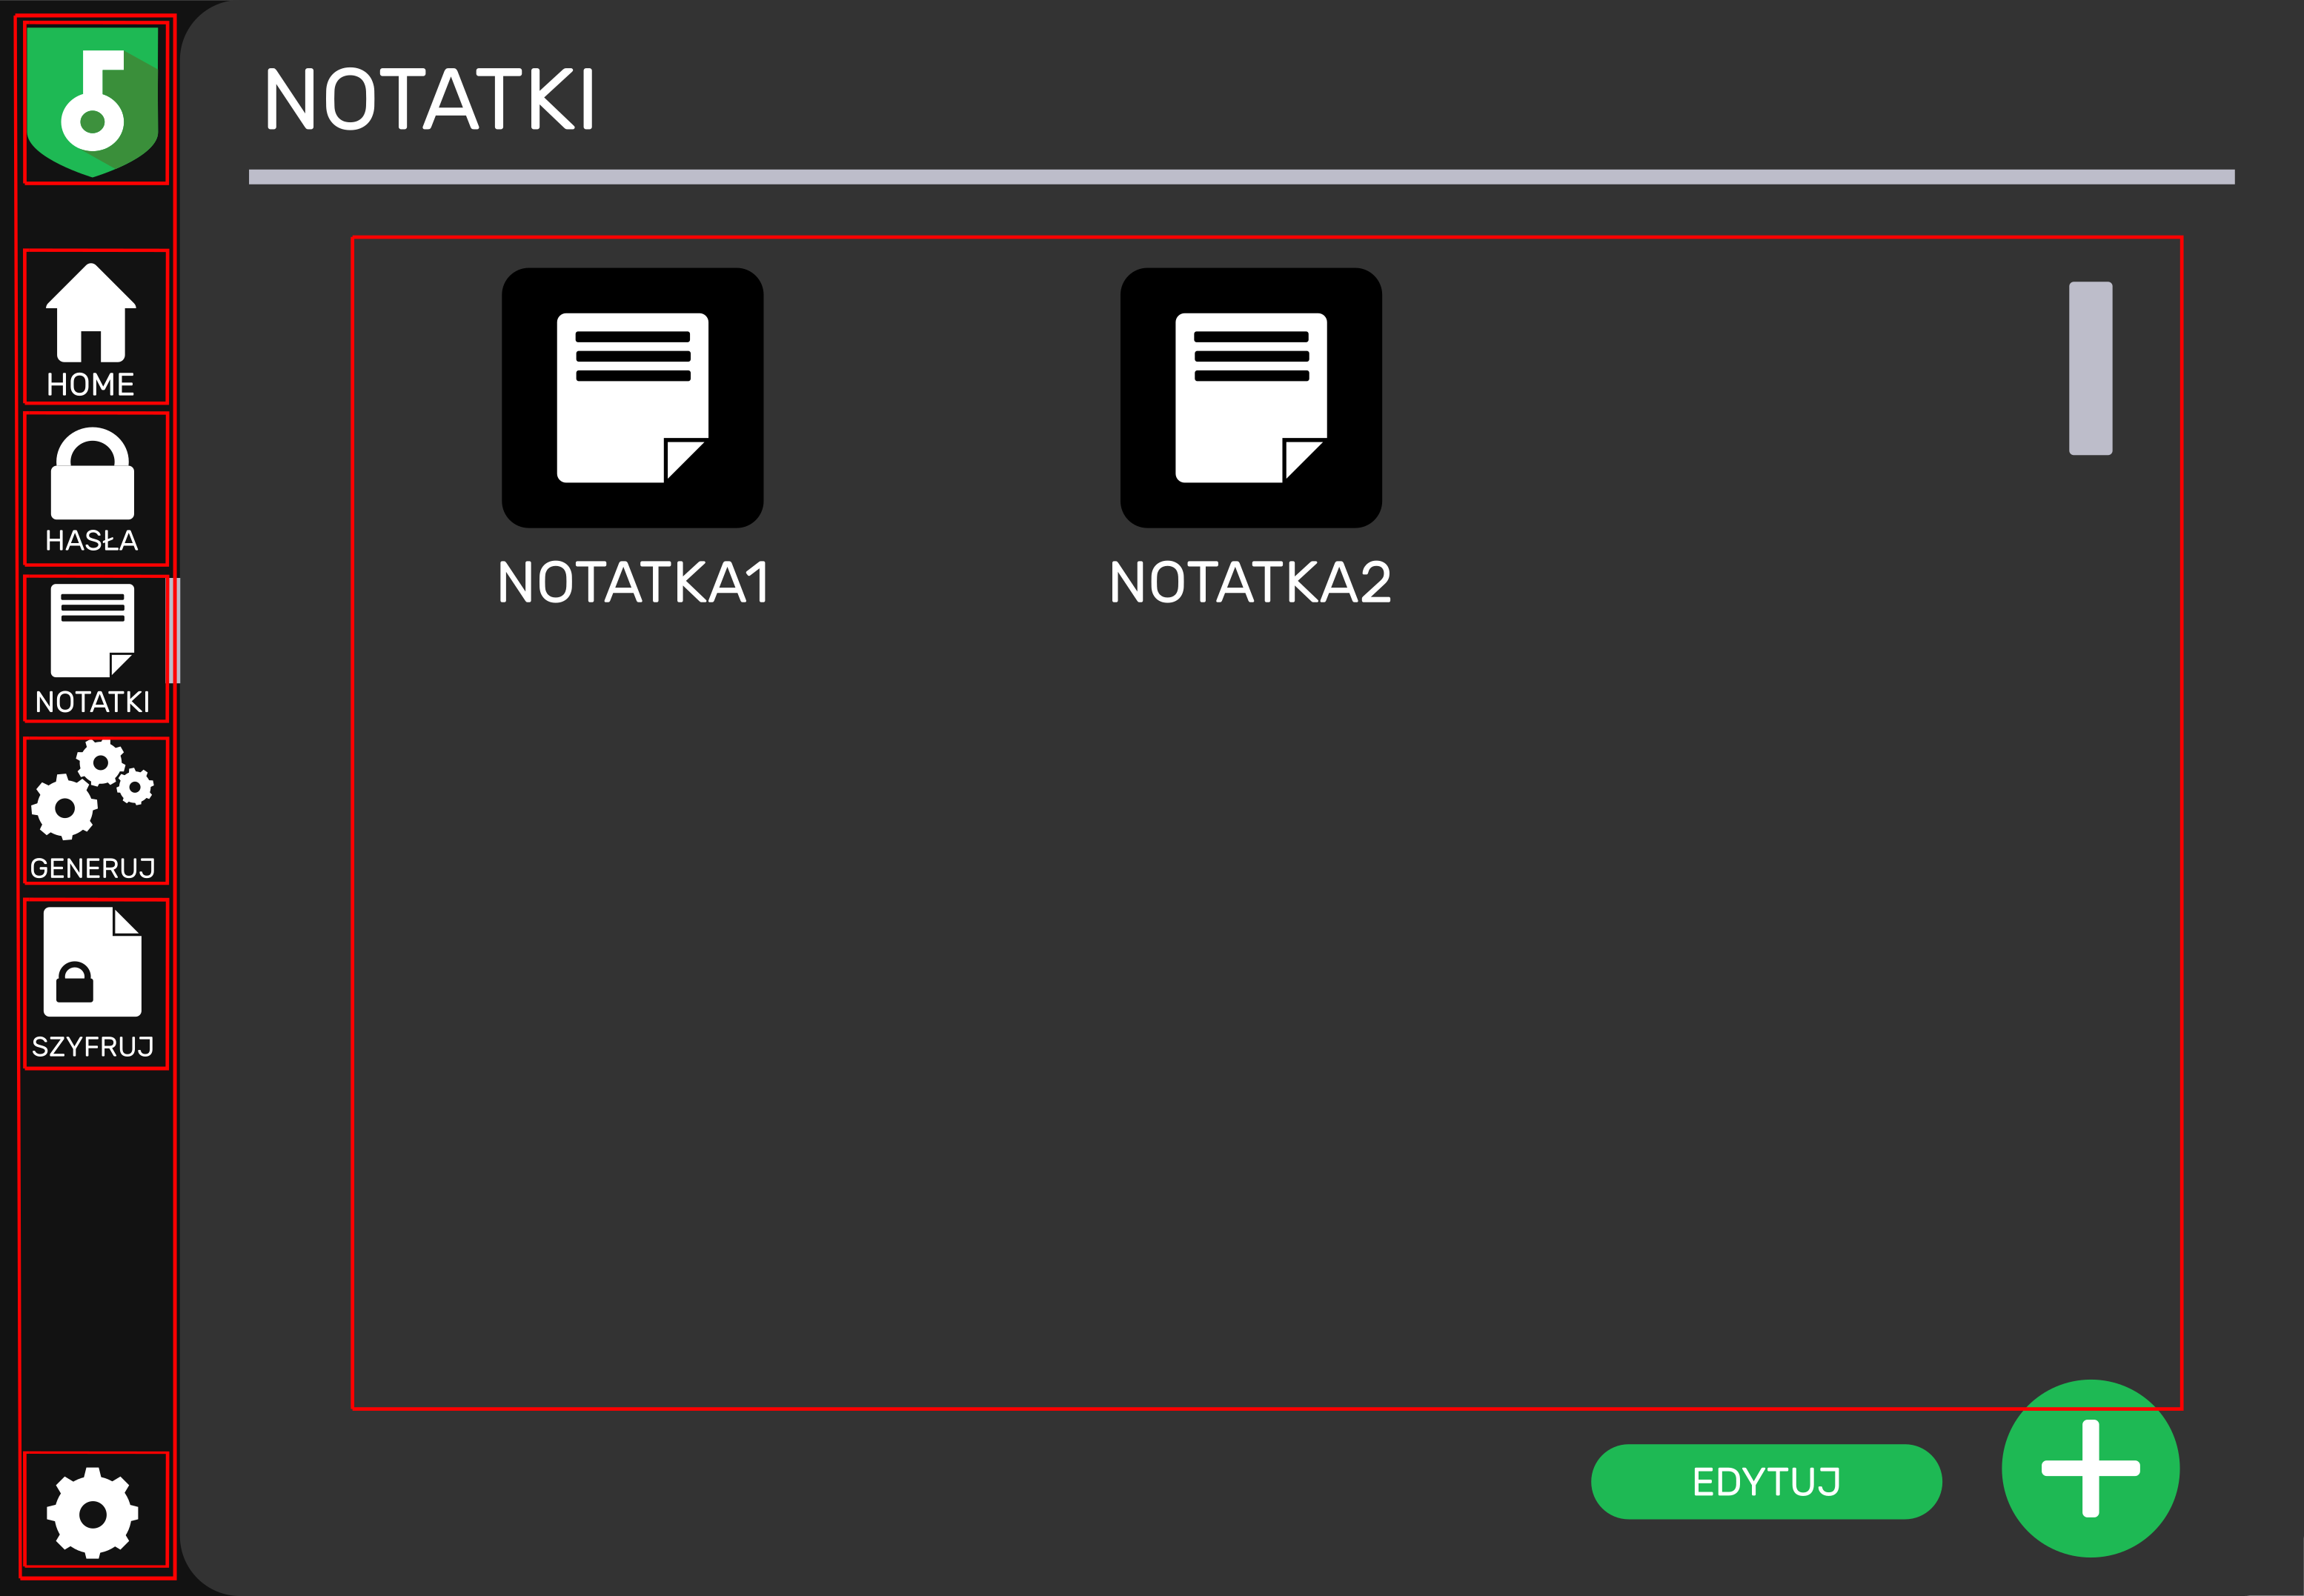
\includegraphics[width=1\textwidth]{img/ekran_notatek.png}
    \caption{Ekran listy notatek}
    \label{fig:notatki}
\end{figure}

\begin{figure}[H]
    \centering
    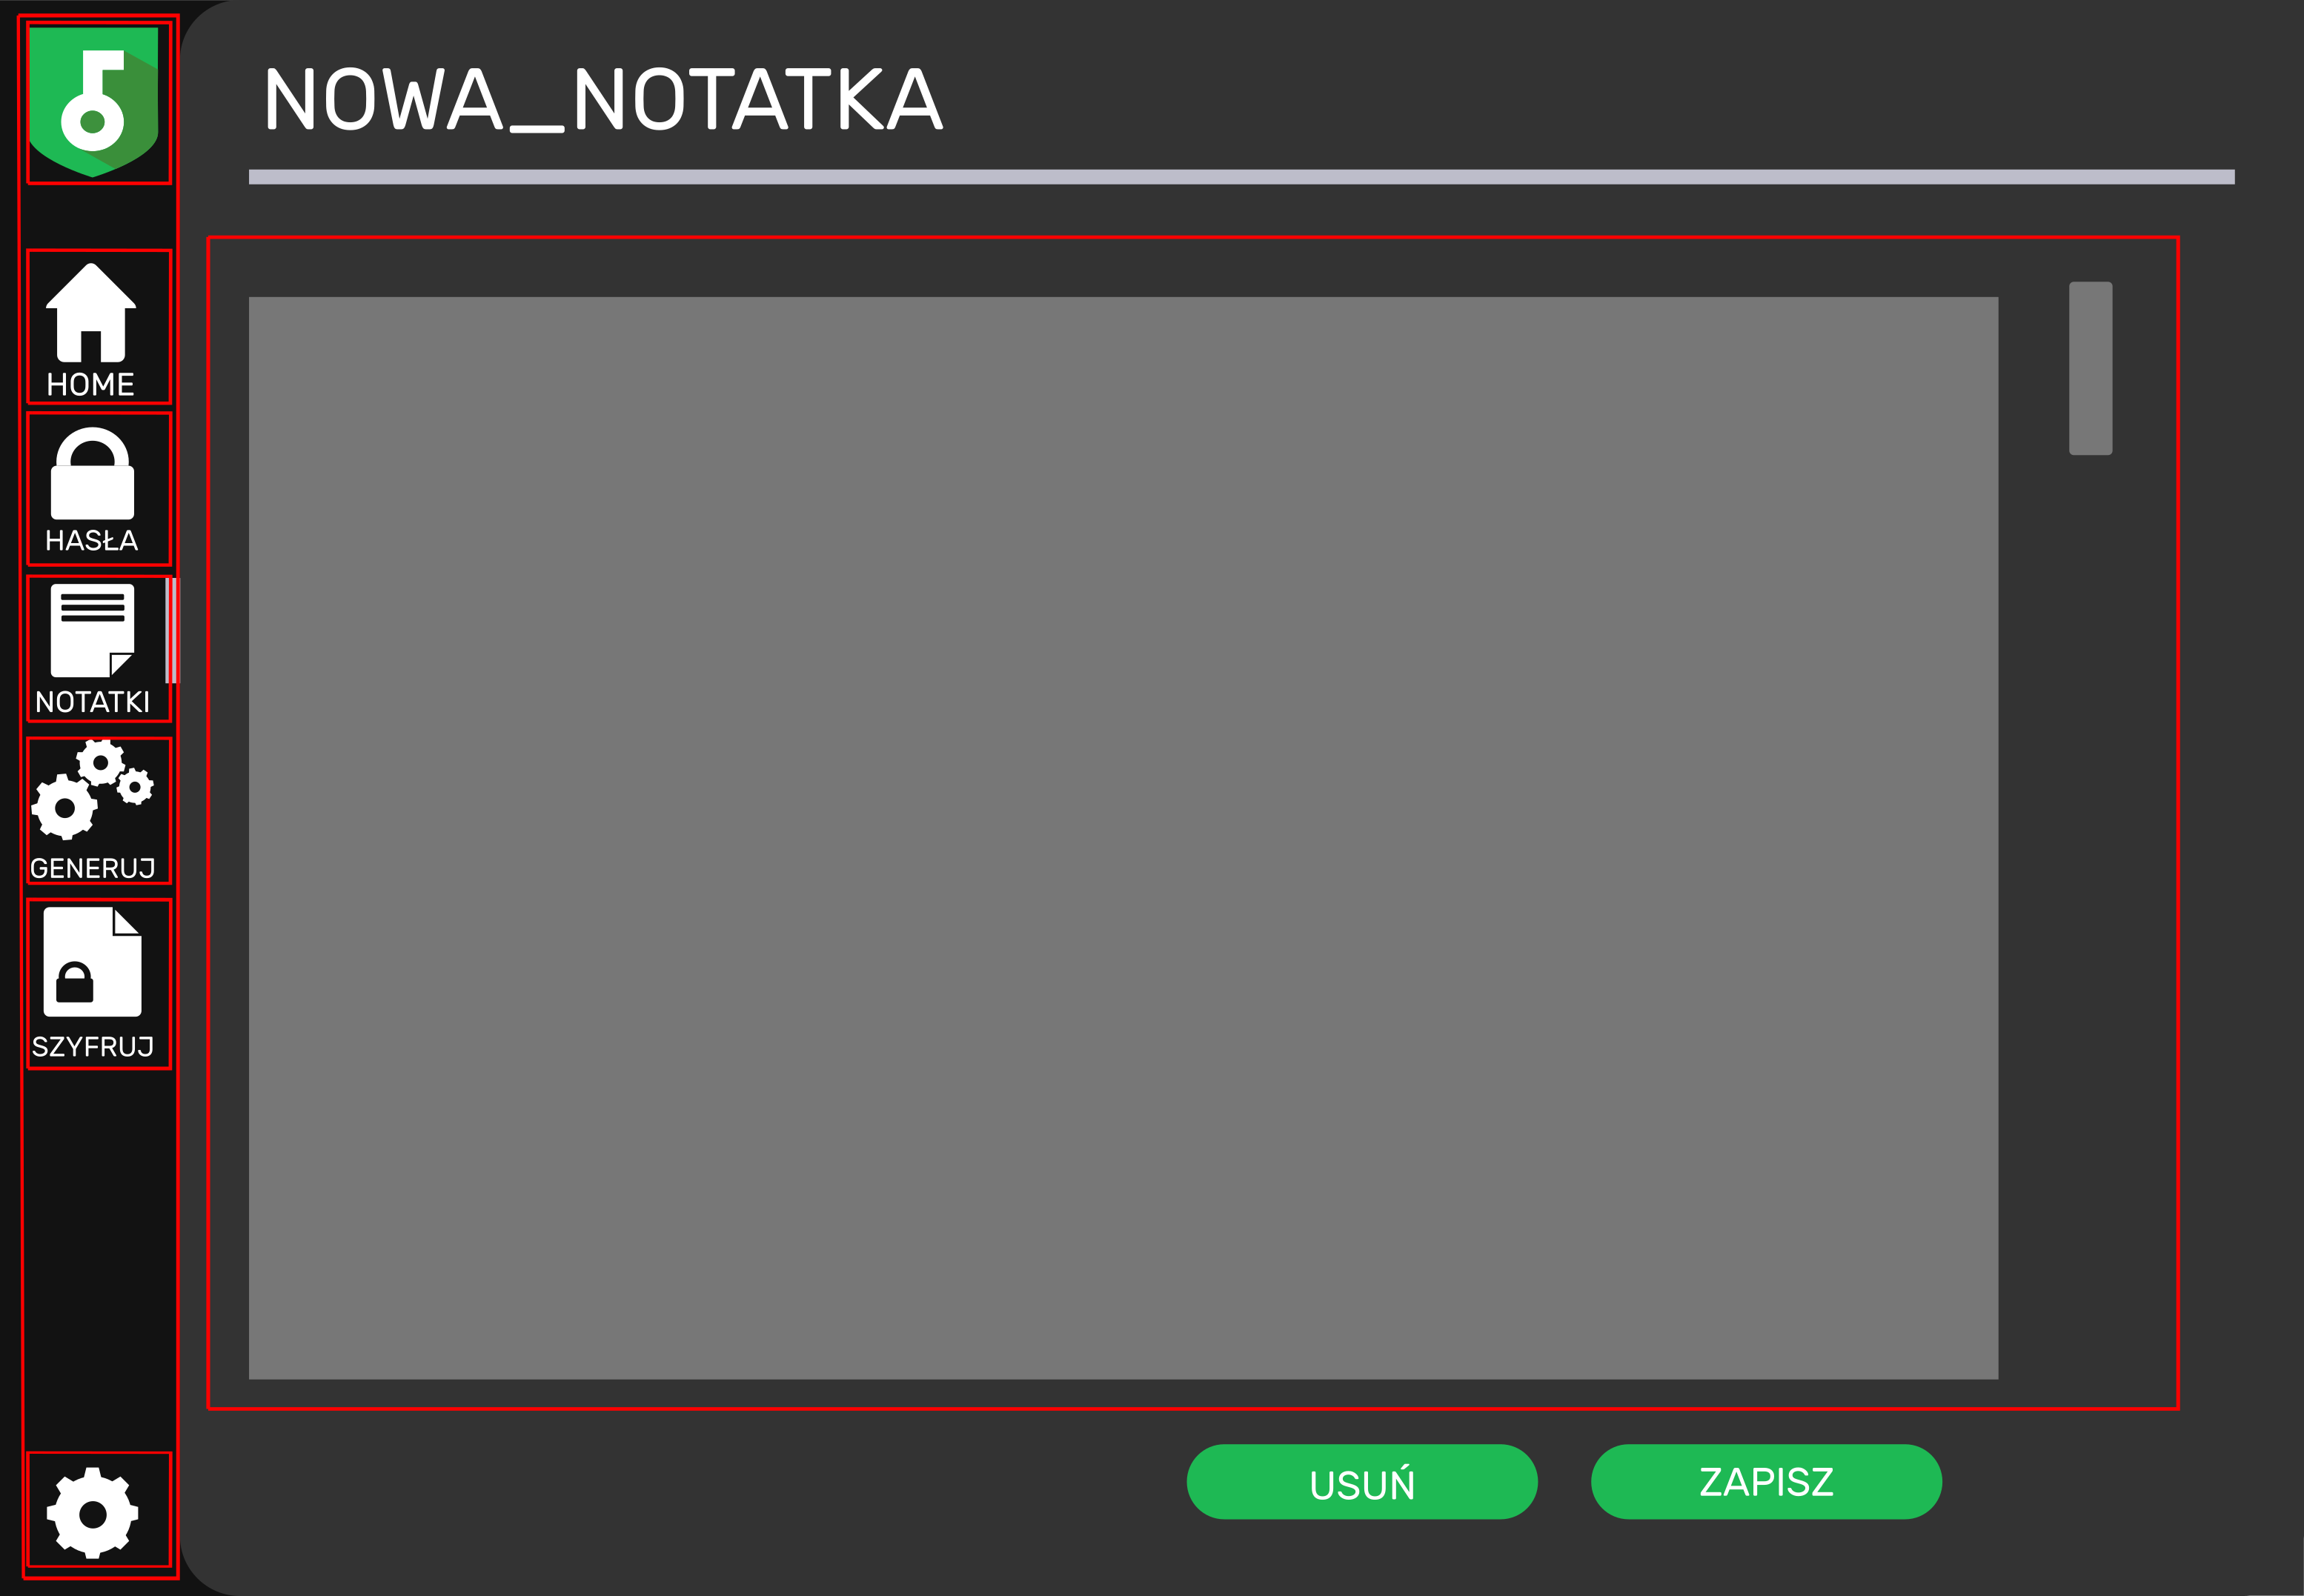
\includegraphics[width=1\textwidth]{img/ekran_nowej_not.png}
    \caption{Ekran dodawania lub edycji notatek}
    \label{fig:notatkNowe}
\end{figure}

\begin{figure}[H]
    \centering
    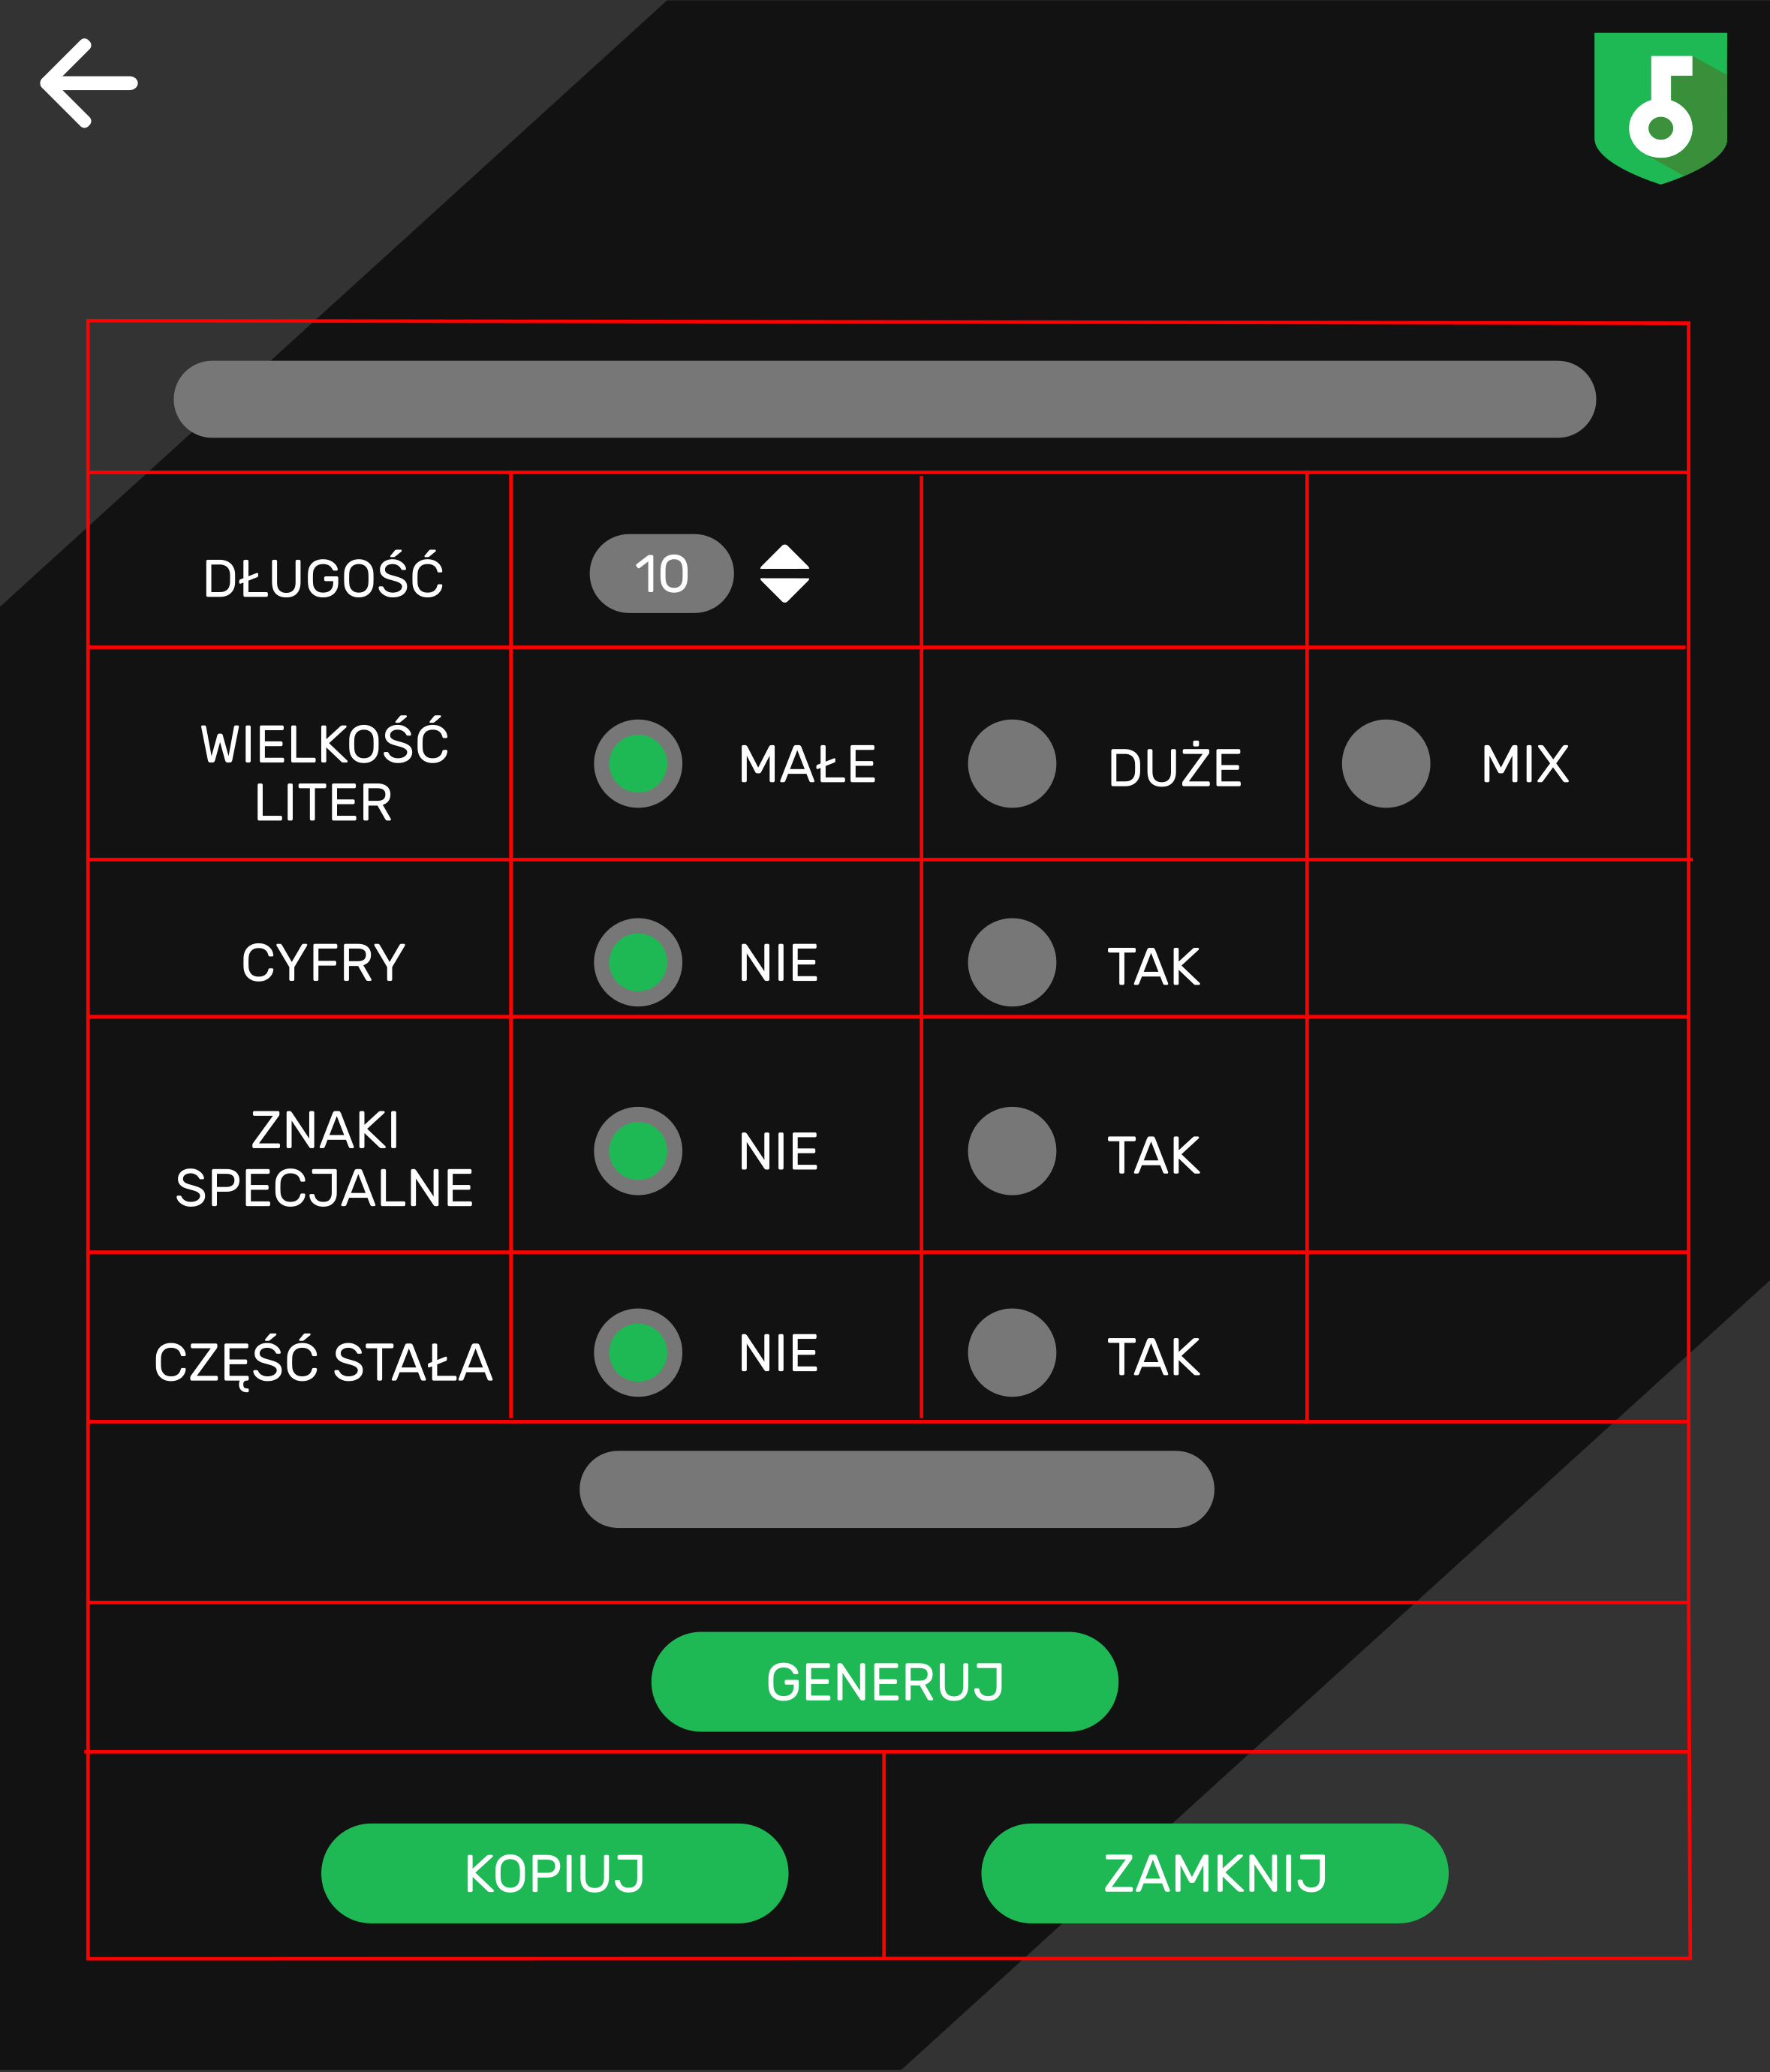
\includegraphics[width=1\textwidth]{img/ekran_generacji.png}
    \caption{Ekran szyfrowania plików podanych przez użytkownika}
    \label{fig:szyfrowanie}
\end{figure}



\section{Testowanie}
\subsection{Użyte narzędzia}
Do przetestowania kodu użyjemy narzędzi z biblioteki AssertJ. Natomiast GUI przetestujemy ręcznie podczas tworzenia aplikacji. Dodatkowo gotowy program przetestujemy sami, grając w niego oraz przekażemy go do testów znajomym.

\subsection{Konwencja}
Metody testujące przyjmą nazwy przypominające równoważniki zdań, aby w~jednoznaczny sposób przekazać informację o badaniu konkretnej funkcjonalności.


\subsection{Warunki brzegowe}
\begin{itemize}
    \item Możliwość otwarcia pliku konfiguracyjnego.
    \item Możliwość otwarcia i zapisu pliku stanu gry.
    \item Odpowiednie działanie programu w przypadku spotkania się wiązki laserowej i spadającego klocka.
    \item Odpowiednie działania programu w kontekście zliczania punktów gracza.
    \item Odpowiednie działanie programu w przypadku spotkania się statków.
\end{itemize}

\section{Diagram klas}
\begin{figure}[H]
    \centering
    \includegraphics[width=\textwidth]{img/diagram-klas.png}
    \caption{Diagram klas}
    \label{fig:diagram}
\end{figure}
\label{end}

\end{document}